\documentclass[a4paper,12pt]{report}
\usepackage[hmargin=2cm, vmargin=2cm]{geometry}
\usepackage[utf8]{inputenc}
\usepackage[T1]{fontenc}
\usepackage[french]{babel}
\usepackage{indentfirst}
\usepackage{graphicx}
\usepackage{color}
\usepackage{float}
\usepackage{fancyvrb}
\usepackage{xcolor}
\usepackage{verbatim}
\usepackage{setspace}
\usepackage{colortbl}
\usepackage[french]{varioref}
\usepackage{amsmath,amssymb}
\usepackage{amsfonts}
\usepackage{url}
\usepackage{here}
\usepackage{multicol}
\usepackage{setspace}
\usepackage{caption}
\usepackage{wrapfig}
\usepackage{subfig}
\usepackage{amsmath}
\usepackage{fancyhdr}
\usepackage{supertabular}
\usepackage{hhline}
\usepackage{array}

\usepackage{multirow}
\usepackage{array}
\newcolumntype{P}[1]{>{\centering\arraybackslash}p{#1}}
\usepackage{longtable}


\usepackage{polyglossia}
\setdefaultlanguage{french}
\setotherlanguage[variant=american]{english}

\usepackage{caption}
\usepackage{lipsum}
\usepackage{pdfpages}   
\usepackage{pgf, tikz}
\usepackage[colorlinks=true,urlcolor=blue,linkcolor= black,citecolor=black]{hyperref}
\usetikzlibrary{arrows,shapes,positioning}

\usepackage[Lenny]{fncychap} % Sonny, Lenny, Glenn, Conny, Rejne, Bjarne
\frenchbsetup{StandardItemLabels=true, CompactItemize=false, ReduceListSpacing=true}
\definecolor{whitesmoke}{rgb}{0.96, 0.96, 0.96}
\newsavebox{\BBbox}
\newenvironment{DDbox}[1]{
\begin{lrbox}{\BBbox}\begin{minipage}{\linewidth}}
{\end{minipage}\end{lrbox}\noindent\colorbox{whitesmoke}{\usebox{\BBbox}} \\
[.5cm]}

\newcommand{\chaptertoc}[1]{\chapter*{#1}
\addcontentsline{toc}{chapter}{#1}
\markboth{\slshape\MakeUppercase{#1}}{\slshape\MakeUppercase{#1}}}

\pagestyle{fancy}
\renewcommand{\headrulewidth}{1pt} 
\fancyhead[L]{\rightmark}%la section \leftmark pour chapitre
\fancyhead[R]{LPHEA}
\newcommand{\reporttitle}{\textcolor{blue}{Titre}}    
\newcommand{\reportauthor}{...}
\newcommand{\reportsubject}{\textbf{Mémoire}\\présenté pour obtenir le diplôme de Master en: \\ %\vspace{0.4cm}
\textbf{Physique des Hautes Énergies, Astrophysique et Physique Computationnelle}} 
\newcommand{\HRule}{\rule{\linewidth}{0.9mm}}
\setlength{\parskip}{1ex} % Espace entre les paragraphes
\let\cleardoublepage\clearpage

\providecommand\textsubscript[1]{\ensuremath{{}_{\text{#1}}}}
\makeatletter
\newcommand\arraybslash{\let\\\@arraycr}
\makeatother
% Footnote rule
\setlength{\skip\footins}{0.0469in}
\renewcommand\footnoterule{\vspace*{-0.0071in}\setlength\leftskip{0pt}\setlength\rightskip{0pt plus 1fil}\noindent\textcolor{black}{\rule{0.25\columnwidth}{0.0071in}}\vspace*{0.0398in}}
\setlength\tabcolsep{1mm}
\renewcommand\arraystretch{1.3}
\title{}

\begin{document}

  \begin{titlepage}

    \begin{figure}[h!]
    \begin{minipage}[b]{0.25\linewidth}
    \begin{center}
    
\includegraphics[width=20mm]{un}
    \end{center}
    
   \end{minipage}\hfill
   \begin{minipage}[b]{0.45\linewidth}   
      \begin{center}
      
\includegraphics[width=40mm]{sem}
      \end{center}
      
   \end{minipage}
   \begin{minipage}[b]{0.27\linewidth}
      \begin{center}
       
\includegraphics[width=33mm]{labo}
      \end{center}
     
   \end{minipage}\hfill
   
\end{figure}
    \begin{center}
    \huge{ Université Cadi Ayyad} \\
    \large  Faculté des Sciences Semlalia\\
    Laboratoire de Physique des Hautes Énergies et Astrophysique
    \end{center}
     \HRule 
 \begin{center}
      
{\large \reportsubject}\\[0.5cm]
\HRule \\[0.4cm]
\Large Sous le thème: \\ \vspace{0.5cm}
{\Huge \bfseries \reporttitle}\\[0.4cm]
\HRule \\[0.8cm]


\begin{Large}
 
   \begin{minipage}[t]{0.45\linewidth}
      \begin{flushleft}
      \emph{Auteur :}\\
    \reportauthor
\end{flushleft}       
   \end{minipage}
    \begin{minipage}[t]{0.45\linewidth}   
      \begin{flushright}
          \emph{Encadrant:} \\
    Pr. ... \textsc{........} \\
    \emph{Co-encadrant:} \\
	Pr. ........... \textsc{..........}
\end{flushright}   
   \end{minipage}\hfill
 
   
 
\end{Large}


\vspace{1cm}

{\large }
 
  \end{center}
  \begin{flushleft}
   Soutenu le .. Juillet 2021 devant la commission d'examen:\\
   \begin{itemize}
    \item ........		\hfill PES, Faculté des Sciences Semlalia, Marrakech
    \item ........		\hfill PES, Faculté des Sciences Semlalia, Marrakech
    \item ........		\hfill PES, Faculté des Sciences Semlalia, Marrakech
    \item ........	   \hfill PES, Faculté des Sciences Semlalia, Marrakech
    \end{itemize}
  \end{flushleft}
  \vfill
   \begin{center}
   \textbf{Année Universitaire 2020 - 2021}
  \end{center}
\end{titlepage}
\tableofcontents{} 
\listoffigures
\listoftables
\chapter*{Remerciements}


\chaptertoc{Introduction Générale}

Contrairement à ce que l'on pense généralement de la physique nucléaire, les propriétés des noyaux ne sont pas encore totalement comprises et le domaine a récemment accompli des progrès majeurs tant d'un point de vue théorique qu'expérimental.

Auparavant, l'étude des noyaux atomiques se limitait aux noyaux stables ou à ceux situés près de la vallée de stabilité. Cependant, au fil des années, Les recherches en physique nucléaire ont été étendues aux noyaux exotiques. Les modèles nucléaires, qui sont essentiellement basés sur des noyx proches de stabilité, divergent à mesure que l'on s'approche des limites de Stabilité. Pour remédier à ce problème plusieurs approches ont été élaborées  pour décrire les noyaux stables et appliquées à certains noyaux exotiques.

Pour les noyaux légers, le nombre relativement petit de nucléons donne la possibilité d’utiliser l’interaction à deux corps pour reproduire les comportements nucléaires, par exemple : calculs ab-initio (fonction de Green - modèle en couches Monte-Carlo). Les noyaux de masse moyenne jusqu’à A ${\sim}$ 60 peuvent être traités par le modèle en couche à grande échelle. Pour les noyaux plus lourds, on utilise des théories de champ moyen soient non relativistes  ou relativistes. 

Les méthodes microscopiques utilisent les théories du champ moyen ont acquis un degré de fiabilité remarquable car ils sont moins compliqués et ils décrivent avec succès les propriétés statiques et dynamiques des noyaux. L'une des approches phénoménologiques les plus importantes, largement utilisée dans les calculs de structure nucléaire, est la méthode Hartree-Fock-Bogoliubov, qui permet de traiter les particules et les trous sur un pied d'égalité en unifiant la description auto-cohérente des orbitales nucléaires, telle qu'elle est donnée par l'approche Hartree-Fock (HF), et la théorie de l'appariement Bardeen-Cooper-Schrieffer (BCS) en une seule méthode variationnelle.

L’objectif de ce travail est d’étudier les propriétés de l’état fondamental de plusieurs chaines isotopiques, allant du côté riche en protons jusqu’au côté riche en neutrons, en utilisant la méthode de Hartree Fock Bogoliubov non relativiste.


\thispagestyle{empty}

 
%

\chapter{  La théorie de HARTREE-FOCK-BOGOLIUBOV}

La théorie Hartree-Fock-Bogoliubov (HFB) est à la fois une extension de la théorie de Hartree-Fock (HF) et de la théorie de Bardeen-Cooper-Schrieffer (BCS). Afin d’avoir une bonne compréhension de cette approche, il est utile de passer en revue un bref résumé de la théorie la plus générale de Hartree-Fock et de la théorie de (BCS) de l''''''''''''''''''''''''''rrappariement.

\section{La théorie de Hartree-fock}

La méthode de \textbf{Hartree-Fock (HF)}  est basée sur l’hypothèse que les nucléons composant le noyau peuvent être considérés comme indépendants dans un champ moyen construit de manière auto-cohérente. Ceci s’explique par la nature quantique des nucléons, le principe de Pauli et la partie fortement répulsive à courte portée de l’interaction nucléon-nucléon. Ainsi, on peut considérer les nucléons comme des particules indépendantes se déplaçant dans un potentiel moyen qu’ils créent eux-mêmes. L’ingrédient de base de ces théories est l’hamiltonien microscopique qui régit la dynamique des nucléons individuels plongés dans un potentiel moyen qu’ils créent collectivement. Cet hamiltonien peut s’écrire sous la forme : 

\begin{equation}H=\sum _{\mathit{ij}} T_{\mathit{ij}} a_i^{+} a_j +\frac {1}{
4} \sum
_{\mathit{ijkl}}V_{\mathit{ijkl}}a_i^{+} a_j^{+}a_k a_l \end{equation}


où le premier terme correspond à l’énergie cinétique et $V_{\mathit{ijkl}}$  l’élément de matrice a deux corps de l’interaction effective. Les opérateurs $a_i^{+?}$ \textit{\ }et  $a_i$  représentent respectivement les opérateurs de création et d’annihilation de fermions dans l’état à un corps $|i\rangle$.

Dans la méthode de \textbf{Hartree-Fock (HF)}  La fonction de l’état fondamental du noyau est recherchée sous la forme d’un déterminant de Slater construit à partir des fonctions d'onde individuelles des nucléons : 
\begin{equation}|\left.\Psi _{\mathit{HF}}\right\rangle
=\mathit{det}\left[\Phi _{\mathit{\alpha 1}}\left(x_1\right).\Phi _{\mathit{\alpha 2}}\left(x_2\right){\dots}\Phi
_{\mathit{\alpha A}}\left(x_A\right)\right]\end{equation}


avec $|\left.\Psi _{\mathit{HF}}\right\rangle $  la fonction d’onde du noyau. Les équations de Hartree-Fock s’obtiennent en minimisant l’énergie totale du noyau :

\begin{equation}E_{\mathit{HF}}=\frac{\left\langle \Psi _{\mathit{HF}}\left|H\left|\Psi _{\mathit{HF}}\right.\right.\right\rangle
}{\left\langle \Psi _{\mathit{HF}}\left|\Psi _{\mathit{HF}}\right.\right\rangle
}\end{equation}

Ce principe variationnel conduit aux équations de \textbf{Hartree-Fock (HF)}  :

\begin{equation}h\Phi _{\beta _i}=\left\{\frac{-\hbar
}{2m}{\nabla}^2+U_{\mathit{HF}}\left[\Phi _{\alpha }\right]\right\}\Phi _{\beta _i}=\varepsilon _{\beta
_i}\quad i=1,{\dots},A\end{equation}


où le champ Hartree-Fock $U_{\mathit{HF}}\left[\Phi _{\alpha }\right]$ dépend lui-même des fonctions d’onde individuelles $\Phi _{\alpha }$  générant ainsi un système auto-cohérent de A équations non-linéaires.

Pour résoudre ce système d’équations, il faudrait déjà connaître la solution ! On procède donc de manière itérative en postulant une solution (fonction test) et en l’injectant dans le système, ce qui permet de construire le premier hamiltonien HF que l’on diagonalise. Les états propres et fonctions propres obtenus sont ensuite utilisés pour reconstruire un nouvel hamiltonien, et ainsi de suite, jusqu’à ce que la variation du jeu de fonctions d’onde entre deux itérations successives soit inférieure à une valeur fixée.

L’approximation de Hartree-Fock est bien adaptée à la description des noyaux pour lesquels il existe, dans le spectre de particules individuelles un écart en énergie ("gap") important entre le dernier niveau occupé et le premier état vide. Ce ”gap” garantit la stabilité du noyau générant un nombre magique pour le nombre de neutrons ou de protons correspondant. C’est le cas des noyaux pairs-pairs à couches fermées. L‘approximation HF est par contre insuffisante dès que l’on veut décrire les états fondamentaux des noyaux situés en milieu de couches pour lesquels l’état fondamental sera quasiment dégénéré avec une multitude d’autres états obtenus à partir de configurations de type particule-trou construites sur ce dernier. L’introduction des corrélations d’appariement permet de restaurer un "gap" en énergie entre états de "quasi-particules", et ainsi de redonner une bonne solution pour l’état fondamental du noyau.

\section{Approximation BCS}

Expérimentalement, tous les noyaux pairs-pairs possèdent un état fondamental de spin nul, ce qui indique que les nucléons ont tendance à se coupler deux à deux dans des états de spin opposé. Une description réaliste des noyaux doit prendre en compte ces corrélations. Ce qui n’est pas le cas dans l’approximation de Hartree-Fock où l’interaction résiduelle de l’appariement est négligée. C’est pourquoi la méthode de Hartree-Fock est généralement utilisée avec l’approximation BCS, proposée par J. Bardeen, L.N. Cooper et J.R. Schrieffer en 1957, qui permet de décrire des corrélations similaires dans la matière condensée supraconductrice. Le concept d’appariement a été introduit en physique de la matière condensée, où, sous l’action d’une interaction attractive (efficace), les électrons peuvent se coupler pour former les paires de Cooper, responsables à basse température du phénomène de supraconductivité. 

Dans la théorie BCS, la fonction d’onde de l’état fondamental d’un système pair-pair est approximée par l’expression suivante :   

\begin{equation}|\left.BCS\right\rangle
=\prod _{k>0}\left(u_k+v_k a_k^{+} a_{\overline k}^{+}\right) | \left.0\right\rangle
\end{equation}


où $k$ et $\overline k$ représentent des états appariés à une seule particule et sont reliés par l’opérateur de renversement du sens de temps, de telle sorte que l’espace des états à un corps est partitionné en des états $k > 0$ et des états  $k< 0.u_k$ et $v_k$ sont les amplitudes d’occupation ($|v^2_k|$ est la probabilité que la paire ($k , \overline k$) soit occupée et$\left|\left.u_k^2\right|+\left|v_k^2\right.\right|=1$ .Le système est donc décrit en terme de paires indépendantes, et non en terme de particules indépendantes. 
L’approximation BCS permet donc un traitement approché des effets d’appariement. Cependant, elle brise une symétrie (celle de la conservation du nombre de particules) qui s’ajoute aux symétries déjà brisées dans l’approximation d’HF, ce qui est un point de défaut. Cette approche présente l’inconvénient de ne pas être adaptée pour le cas des noyaux impairs. Il est nécessaire de la généraliser selon la méthode de Hartree Fock Bogoliubov(HFB).

\section{La transformation de Bogoliubov}

Pour tenir compte des effets d’appariement dans le noyau, on introduit le concept de quasi-particules de  Bogoliubov dans la méthode hartree-fock. On transforme ainsi l’état HF de particules indépendantes  $\left\{a,a^{+}\right\}$  en un état Hartree-Fock-Bogoliubov (HFB) de quasi-particules indépendantes $\left\{\beta,\beta^{+}\right\}$  en utilisant la transformation suivante :

\begin{equation}\beta _{\alpha }=\sum_{i} U_{\mathit{i\alpha }}^{\ast }a_i+V_{\mathit{i\alpha }}^{\ast
}a_i^{+}\end{equation}


\begin{equation}\beta _{\alpha }^{+} =\sum
_iU_{\mathit{i\alpha }}a_i^{+} + V_{\mathit{i\alpha
}}a_i\end{equation}



ou sous la forme matricielle 

\begin{equation}\left(\begin{matrix}\beta
\\\beta
^{+}\end{matrix}\right)=\left(\begin{matrix}U^{+}&V^{+}\\V^T&U^T\end{matrix}\right)\left(\begin{matrix}a\\a^{+}\end{matrix}\right)=w^{+}\left(\begin{matrix}a\\a^{+}\end{matrix}\right)\end{equation}


Les éléments de matrice \textit{U} et \textit{V}  satisfont aux relations : 

\begin{equation}U^{+} U+V^{+} V=1 \quad UU^{+}+V^{\ast }V^T=1\\ U^TV+V^TU=0 \quad UV^{\ast }+V^{\ast }U^T=0\end{equation}
    
  

\section{ La méthode Hartree fock-bogoliubov}
Dans l’approximation HFB, l’hamiltonien est essentiellement réduit à deux potentiels : le potentiel moyen auto-cohérent $\Lambda $  de la théorie de Hartree-Fock, et un champ d’appariement supplémentaire $\Delta $, connu de la théorie BCS.

L’état HFB, noté $|\Phi\rangle$, est défini comme le vide associé aux opérateurs d’annihilation de quasi-particules $\beta_i$. Il vérifie donc, pour tout $i$ :$\beta _i |\left.\Phi \right\rangle =0$

On impose de plus à cet état d’être normé :       
\begin{equation}\left\langle \Phi \left|\Phi \right.\right\rangle
=0\end{equation}
           
L’hamiltonien à deux corps peut s'écrive comme une somme de deux termes : l'énergie cinétique $t_{ij}$ et les éléments de matrice d'interaction antisymétrique à deux corps $V_{ijkl}$. Ainsi, en deuxième quantification, cet hamiltonien prend la forme :
\begin{equation}H=\sum
_{\mathit{ij}}T_{\mathit{ij}}a_i^{+}a_j+\frac 1 4\sum
_{\mathit{ijkl}}V_{\mathit{ijkl}} a_i^{+}a_j^{+}a_k a_l\end{equation}


avec $v_{ijk}$, les éléments de matrice de l’interaction NN antisymétrique :

\begin{equation}v_{\mathit{ijkl}}=\left\langle \mathit{ij}\left|v\left|\mathit{kl}\right.\right.\right\rangle -\left\langle
\mathit{ij}\left|v\left|\mathit{lk}\right.\right.\right\rangle\end{equation}


Pour un état HFB  $| \Phi \rangle $ donné, l’énergie moyenne E\textsubscript{HFB} de cette configuration sera donnée par :

\begin{equation}E_{\mathit{HF}B}=\left\langle \Phi \left|H\left|\Phi \right.\right.\right\rangle =\sum
_{\mathit{ij}}t_{\mathit{ij}}\rho _{\mathit{ij}}+\frac 1 2\sum _{\mathit{ijkl}}v_{\mathit{ijkl}}\left[\rho
_{\mathit{ki}}\rho _{\mathit{lj}}+\frac 1 2k_{\mathit{ij}}^{\ast }k_{\mathit{kl}}\right]\end{equation}


où $\rho $ est la matrice densité du système, définie par :
\begin{equation}\rho =\left\langle \Phi
\left|a_j^{+}a_i\left|\Phi \right.\right.\right\rangle =\sum _mV_i^{m\ast
}V_j^m\end{equation}


Le terme $K$ est le tenseur d’appariement (ou densité anormale) définie par :

\begin{equation}K_{\mathit{ij}}=\left\langle \Phi
\left|a_j^{+}a_i\left|\Phi \right.\right.\right\rangle =\sum _mV_i^{m\ast
}U_j^m\end{equation}


Le terme en $K*K$, dans l’équation de l’énergie $E_{HFB}$, représente la contribution des corrélations d’appariement à l’énergie. Dans la limite où l’appariement est nul, on retrouve l’énergie moyenne de la théorie HF.
Il est également utile de définir la matrice densité généralisée, notée R, qui permet de regrouper la matrice densité a un corps $\rho$, et le tenseur d’appariement $k$, en une seule matrice. Elle est définie comme :
\begin{equation}R=\left(\begin{matrix}\rho
&k\\-k^{\ast }&1-\rho ^{\ast
}\end{matrix}\right)\end{equation}


On minimise l’énergie $E_{HFB}$ de la même manière que pour HF, en utilisant un principe variationnel. On obtient alors les équations HFB qui s’écrivent sous forme matricielle :
\begin{equation}H_{\mathit{HFB}}=\left(\genfrac{}{}{0pt}{0}{u_i}{v_i}\right)=\left(\begin{matrix}h&{\Delta}\\-{\Delta}^{\ast
}&-h^{\ast
}\end{matrix}\right)\left(\genfrac{}{}{0pt}{0}{u_i}{v_i}\right)=E_i\left(\genfrac{}{}{0pt}{0}{u_i}{v_i}\right)\end{equation}


\begin{equation}H_{\mathit{HFB}}=\left(\genfrac{}{}{0pt}{0}{u_i^{\ast }}{v_i^{\ast
}}\right)=\left(\begin{matrix}h&{\Delta}\\-{\Delta}^{\ast }&-h^{\ast
}\end{matrix}\right)\left(\genfrac{}{}{0pt}{0}{u_i^{\ast }}{v_i^{\ast }}\right)=E_i\left(\genfrac{}{}{0pt}{0}{u_i^{\ast
}}{v_i^{\ast }}\right)\end{equation}


où h est le champ particule-trou (champ Hartree-Fock) :
\begin{equation}h_{\mathit{ik}}=t_{\mathit{ik}}+\sum _{\mathit{jl}}v_{\mathit{ijkl}}\rho
_{\mathit{lj}}\end{equation}


Et représente le potentiel d'appariement :
\begin{equation}{\Delta}_{\mathit{ik}}=\frac 1 2\sum
_{\mathit{kl}}v_{\mathit{ijkl}}K_{\mathit{kl}}\end{equation}


Pour conclure, la théorie HFB permet, grâce à la prise en compte des corrélations d’appariement, d’améliorer la fonction d’onde approchant l’état fondamental dans les noyaux non magiques, et ceci en régénérant un gap au-dessus du niveau de Fermi similaire à celui observé dans les noyaux magiques à l’approximation HF à travers une transformation de Bogoliubov.



% Please add the following required packages to your document preamble:
% \usepackage{longtable}
% Note: It may be necessary to compile the document several times to get a multi-page table to line up properly

%% https://www.tablesgenerator.com/latex_tables






\chaptertoc{Résumé}

Dans le but de comprendre la nature de la structure nucléaire, il est devenu essentiel d'explorer et
d'étudier non seulement le comportement des noyaux stables de la charte nucléaire, mais aussi ceux exotiques qui se
trouvent loin de la vallée de stabilité. Les expériences menées sur les noyaux stables ne suffisent pas pour tester
l'universalité des modèles nucléaire. Seule une étude systématique au voisinage des noyaux exotiques, le long d'une
chaîne isotopique, permet d'apporter de nouvelles contraintes sur l'évolution de la structure nucléaire.
 Dans ce mémoire, nous étudions les propriétés de l'état fondamental de certains noyauxsuper-lourds
éloignés de la stabilité pour les chaînes isotopiques à savoir : les isotopes
de\textcolor[rgb]{0.1254902,0.12941177,0.13333334}{~Flérovium} (Fl,
Z=114),\textbf{\textcolor[rgb]{0.1254902,0.12941177,0.13333334}{
}}\textcolor[rgb]{0.1254902,0.12941177,0.13333334}{Livermorium }(Lv, Z=116) et L'oganesson (Og, Z=118) en utilisant
L'approche non relativiste de Hartree-Fock-Bogoliubov (HFB) avec la force de Skyrme SLy4. Les propriétés étudiées sont
: l'énergie de liaison, l'énergie de séparation d'un et de deux neutrons, le rayon des protons et des neutrons,
L'énergie d'appariement et le spectre d'énergie. Les résultats obtenus ont été comparés avec les données expérimentales
disponibles et avec les prédictions des autres modèles théoriques tels que : le modèle de la gouttelette liquide à
portée finie (FRDM), le modèle du champ moyen relativiste (RMF) et l'expérience de Skyrme.


\chaptertoc{Introduction}

 Contrairement à ce que l'on pense généralement de la physique nucléaire, les propriétés des noyaux ne sont
pas encore totalement comprises et le domaine a récemment accompli des progrès majeurs tant d'un point de vue théorique
qu'expérimental.
 Auparavant, l'étude des noyaux atomiques se limitait aux noyaux stables ou à ceux situés près de la vallée
de stabilité. Cependant, au fil des années, \textcolor[rgb]{0.1254902,0.12941177,0.14117648}{Les recherches en physique
nucléaire ont été étendues aux noyaux exotiques qui }présentent de nouveaux comportements et des phénomènes très
inattendus par rapport à la vision standard de la structure nucléaire\textcolor[rgb]{0.1254902,0.12941177,0.14117648}{.
Ces noyaux ont une courte durée de vie, ce qui rend leur étude e}xpérimentale difficile. Même si elles peuvent être
observées, on ne connaît même pas leurs propriétés de base telles que la masse, la forme, la demi-vie et les états
d'excitation les plus bas.
 Les modèles nucléaires, qui sont essentiellement basés sur des noyaux proches de stabilité, divergent à
mesure que l'on s'approche des limites de Stabilité {\textquotedbl}dri-plines{\textquotedbl}. Pour remédier à ce
problème plusieurs approches ont été élaboréespour décrire les noyaux stables et appliquées à certains noyaux
exotiques.
 Pour les noyaux légers, le nombre relativement petit de nucléons donne la possibilité d'utiliser
l'interaction à deux corps pour reproduire les comportements nucléaires, par exemple : calculs ab-initio (fonction de
Green - modèle en couches Monte-Carlo). Les noyaux de masse moyenne jusqu'à A ${\sim}$ 60 peuvent être traités par le
modèle en couche à grande échelle. Pour les noyaux plus lourds, on utilise des théories de champ moyen soient non
relativistesou relativistes.
 Les méthodes microscopiques utilisent les théories du champ moyen ont acquis un degré de fiabilité
remarquable car ils sont moins compliqués et ils décrivent avec succès les propriétés statiques et dynamiques des
noyaux. L'une des approches phénoménologiques les plus importantes, largement utilisée dans les calculs de structure
nucléaire, est la méthode Hartree-Fock-Bogoliubov (HFB), qui permet de traiter les particules et les trous sur un pied
d'égalité en unifiant la description auto-cohérente des orbitales nucléaires, telle qu'elle est donnée par l'approche
Hartree-Fock (HF), et la théorie de l'appariement Bardeen-Cooper-Schrieffer (BCS) en une seule méthode variationnelle.
 L'objectif de ce travail est d'étudier les propriétés de l'état fondamental de plusieurs chaines
isotopiques, allant du côté riche en protons jusqu'au côté riche en neutrons, en utilisant la méthode de Hartree Fock
Bogoliubov non relativiste.
\thispagestyle{empty}



\chapter{Généralités sur la structure nucléaire}

\section{Le noyau atomique}

 La recherche de la structure nucléaire a commencé avec la première observation de la radioactivité. En
1911, Ernest Rutherford à découvert qu'au cœur de chaque atome se trouve un noyau.
 Le noyau atomique est constitué de A nucléons avec A = N + Z, où A est le nombre de masse, N et Z sont
respectivement les nombres de neutrons et de protons. Ces derniers sont maintenus ensemble par la force nucléaire
forte. Bien que Le noyau ne représente que moins de 0,01\% du volume de l'atome. Mais il contient généralement plus de
99,9\% de sa masse. Les propriétés chimiques d'une substance sont déterminées par les électrons chargés négativement
qui entourent le noyau.
 Il est très fréquent de tracer tous les nucléides connus avec le nombre de neutrons sur l'axe des
abscisses et le nombre de protons sur l'axe des ordonnées pour obtenir la dite «charte nucléaire» ou “nuclear
landscape” (Fig. 1.1).
 La charte nucléaire (Fig. 1.1) montre plusieurs milliers de noyaux qui devraient être liés par la
force forte. La région noire montre les noyaux stables, non radioactifs ou à longue durée de vie, avec des demi-vies
comparables ou plus longues que l'âge de la terre. Il y a moins de 300 de ces espèces et ils constituent ce qu'on
appelle {\textquotedbl}\textit{la vallée de la stabilité}{\textquotedbl}. Les noyaux légers sont stables si le nombre
de protons et le nombre de neutrons sont approximativement égaux. En augmentant le nombre de masse, le nombre de
neutrons doit être plus grand que celui de protons afin d'équilibrer la force de répulsion coulombienne entre les
protons. En outre, les noyaux avec N ou Z égal à certains nombres montrent une stabilité spéciale : les nombres
magiques (Ceux qui marquent les lignes rouges horizontales et verticales sur la figure 1.1). Ces noyaux sont de forme
sphérique avec des couches nucléaires externes fermées. Alors que d'autres noyaux trouvés loin de la vallée de la
stabilité sont également liés, mais ne sont pas complètement stables. Les noyaux avec un excès ou une déficience des
neutrons par rapport à la vallée de la stabilité sont instables et donc ils se désintègrent. La région jaune autour de
la zone de stabilité de la figure 1. 1 indique les noyaux artificiels produits dans les laboratoires avec de courtes
demi-vies. Des milliers de noyaux radioactifs avec des rapportsdeneutrons àprotonstrès petitsou très
\ grandssontencore à
 
 
 
 
 \begin{figure}[htb]
 	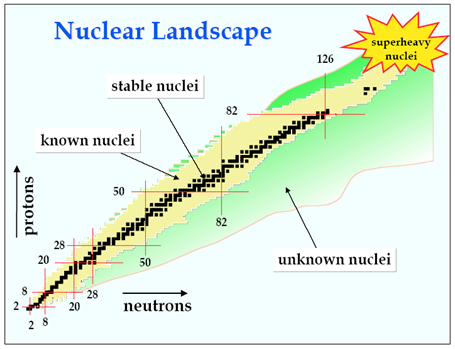
\includegraphics[width=\textwidth]{Chapitre201-img/Chapitre201-img001.png}
 	\caption{Charte des noyaux en
 		fonction du nombre de neutrons et de protons. Elle montre la vallée de la stabilité des particules et les
 		limites de l'existence nucléaire, ou {\textquotedbl}drip-lines{\textquotedbl}}
 \end{figure}
 
  

explorer, c'est la zone des noyaux instables indiquée en vert sur la figure 1.1 appelée«Terra Incognita»,
c'est-à-dire en latin «Terre inconnue». En ajoutant des protons ou des neutrons, nous nous éloignons de la vallée de la
stabilité, et nous atteignons les limites de la stabilité des particules nucléaires, appelées les
{\textquotedbl}drip-lines{\textquotedbl} où la liaison nucléaire se termine, les forces entre les protons et les
neutrons ne sont plus assez fortes pour les maintenir ensemble. La drip-line des protons est déjà déterminée
expérimentalement jusqu'au Protactinium (Pa, Z = 9). Tandis que la drip-line des neutrons est
considérablement plus éloignée de la vallée de lastabilité et plus difficile à approcher et elle n'a été déterminée
\ que jusqu'à l'Oxygène (O, Z = 8). La différence de largeur des drip-lines des protons et des neutrons par rapport à
la ligne de stabilité s'explique par la force de répulsion de Coulomb, qui devient plus grande à mesure que plus de
protons sont ajoutés.
\section{}{Production des noyaux exotiques}
 Les noyaux à durée de vie limitée, instables, radioactifs, sont dits exotiques lorsqu'ils
développent des structures inhabituelles (grande extension de matière, halo ou peau de neutrons, couches présentant de
nouveaux nombres magiques.  Le développement de techniques expérimentales de plus en plus performantes permet
désormais de produire et d'étudier la structure de ces noyaux.
 Diverses réactions nucléaires dans une large gamme d'énergie sont utilisées pour la production de noyaux
radioactifs. Les faisceaux primaires les plus couramment utilisés sont les neutrons, les protons, les deutons et les
ions lourds, leur énergie varie des énergies thermiques aux énergies relativistes. Après la phase de production, les
noyaux exotiques sont manipulés et préparés pour l'expérience. L'ensemble du processus doit être très rapide à cause de
lademi-vie extrêmement courte de ce type des noyaux.


 \begin{figure}[htb]
 	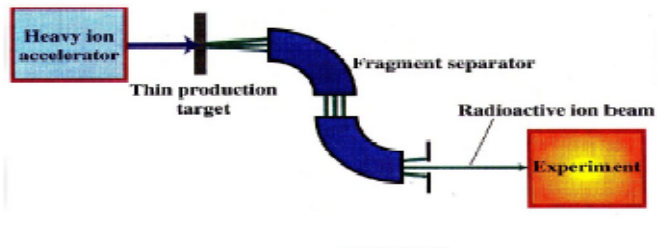
\includegraphics[width=\textwidth]{Chapitre201-img/Chapitre201-img002.png}
 	\caption{Schéma d'une expérience visant à produire les noyaux exotiques.
}
 \end{figure}



Dans le cas d'une réaction de fragmentation, les noyaux exotiques se produit en bombardant une cible avec le faisceau
d'ions stables; l'interaction entre les ions projectiles et ceux de la cible donne naissance à une grande variété de
noyaux, dont de nombreux exotiques. Comme la création d'un noyau exotique spécifique ne se produit que pour un noyau
incident sur dix mille a un million, on comprend alors qu'il faut atteindre les plus hauts flux d'ions incidents
produits pour accroitre la production d'ions secondaires.
\section{Les modèles nucléaires}
 Après l'avènement de la physique nucléaire dans les années 30 par la découverte d'un noyau atomique chargé
en 1911, et l'identification du proton quelques années plus tard, il a fallu attendre 1932 pour que Chadwick mette en
évidence l'existence\textbf{ }du neutron . Une fois les constituants du noyau ont été identifiés, les physiciens ont
alors commencé à proposer des modèles théoriques pour décrire ses propriétés statiques et dynamiques. La plupart de ces
modèles sont souvent utilisés localement pour décrire une région spécifique de la charte nucléaire. Tout d'abord, il y
avait le modèle de la goutte liquide offrant une description satisfaisante des masses et également capable de donner
une première interprétation à la fission des noyaux. Cependant, Ce modèle ne permet toutefois pas d'expliquer certaines
propriétés plus fines des noyaux (niveaux d'énergie des nucléons, transitions nucléaires, nombres magiques,...), ce que
font mieux des modèles dits à particules indépendantes.
 Dans ce qui suit, certains des modèles précurseurs et plus récents représentant le noyau seront brièvement
décrits afin de présenter quelques concepts et formalismes.
\section{1Modèle de la goutte liquide }
\textbf{ }Le modèle de la goutte liquide (LDM) a été historiquement le premier modèle proposé pour
expliquer les différentes propriétés du noyau. Malgré son ancienneté et sa simplicité, il permet d'excellentes
prédictions pour les masses des noyaux. C'est également le premier modèle à donner une interprétation de la fission.
Dans ce modèle semi-empirique, le noyau est interprété comme une sphère de liquide visqueux incompressible de rayon R
proportionnel à la racine cubique du nombre A de nucléon, composé de nucléons interagissant via l'interaction nucléaire
et coulombienne (pour les protons). L'énergie de liaison totale dépend du nombre de protons et neutrons Z et N :
 \begin{equation}B\left(N,Z\right)=a_vA+a_sA^{2/3}+a_c\frac{Z^2}{A^{1/3}}+a_a\frac{(N-Z)^2} A+\delta
(A)\end{equation}
Cette expression constitue la formule de Bethe et Weizsäcker, obtenue en 1935. Elle fournit l'énergie de liaison d'un
noyau quelconque dans un état fondamental. Les termes \textit{a}\textit{\textsubscript{v}},
\textit{a}\textit{\textsubscript{s}}, \textit{a}\textit{\textsubscript{c}} et \textit{a}\textit{\textsubscript{a}}
correspondent respectivement aux coefficients d'énergie de volume, de surface, coulombienne et d'asymétrie, Les valeurs
de ces coefficients sont ajustées sur des masses mesurées. Elles sont données, ci-dessous, en MeV :
 \begin{equation}a_v=-15.7;a_s=18.6;a_c=0.7;a_s=28.1\end{equation}
La signification physique de la formule (1.1) est la suivante :
 Le premier terme est appelé généralement terme de volume, parce qu'il est proportionnel à A (${\propto}$
R\textsuperscript{3}). C'est le terme principal qui résulte des forces d'interaction nucléaire (attractives). En raison
de la saturation de ces forces, l'énergie de liaison qui en résulte est la même pour tous les nucléons. Le coefficient
a\textsubscript{v} correspond donc à l'énergie de liaison moyenne par nucléon, B/A ${\approx}$ +16 MeV.
 Le second terme est proportionnel à A\textsuperscript{2~/3}(${\propto}$ R\textsuperscript{2}), il est donc
appelé le terme de surface. Il traduit le fait que les nucléons en surface sont moins liés, puisqu'ils ont un nombre de
voisins plus faible. On peut calculer à partir de paramètre \textit{a}\textit{\textsubscript{s}} la tension
superficielle $\sigma $définie comme l'énergie de surface par unité de surface.
 \begin{equation}\sigma =\frac{a_s}{4\pi r_0^2}=1.03\mathit{MeV.}\mathit{fm}^{-2}\end{equation} , avec
 \begin{equation}r_0=1.3\mathit{fm}\end{equation}
 Le troisième terme décrit la répulsion colombienne entre les protons qui tend à diminuer l'énergie de
liaison. On peut la calculer approximativement en supposant que les charges sont uniformément distribuées sur une
sphère. L'énergie colombienne d'un tel système est proportionnelle au nombre de paires de protons (${\propto}$
Z\textsuperscript{2}).
 Le quatrième terme représente le terme d'asymétrie. Il décrit la différence d'énergie créée par des
nombres non égaux de neutrons et de protons. En effet, \textcolor[rgb]{0.1254902,0.12941177,0.13333334}{~les noyaux
sont plus stables quand le nombre de neutrons et de protons est identique (si on néglige l'effet de la répulsion
électrostatique).} Pour comprendre l'effet d'un excès de neutrons sur
ce terme, on suppose qu'une situation d'équilibre (N = Z) est perturbée par la transformation de protons en neutrons,
et vice versa. Le nombre de protons ainsi convertis sera N - Z.
Pour chaque conversion, l'énergie de liaison diminue d'une quantité proportionnelle à la différence fractionnaire entre
les niveaux les plus élevés de neutrons et de protons occupés.
 Le dernier terme $\delta $(A) favorisera en énergie les noyaux à nombres pairs de neutrons et protons et
pénalisera les autres cas possibles. Il permet de prendre en compte les corrélations d'appariement :
 \begin{equation}\delta
\left(A\right)=\left\{\begin{matrix}+34A^{-2/3}\text{  pour les noyaux pairs-pairs},\\0\text{  pour les noyaux pairs-impairs},\\-34A^{-2/3}\text{  pour les noyaux impairs -impairs.}\end{matrix}\right.\end{equation}

La figure 1.3 représente les contributions des différents termes, à part celui d'appariement, dans la formule de masse
1.1. Nous pouvons voir que, lorsque A augmente, le terme de surface perd son importance en faveur du terme coulombien.
L'énergie de liaison a un large maximum au voisinage de A ${\propto}$ 56 ce qui correspond aux isotopes de Z pair du
fer et du nickel.
\subsection{ Modèle en couches}

\textbf{1.4.2.1 Nombres magiques}

En observant de plus près les énergies de liaison des nucléides, on trouve que les noyaux ayant des nombres pairs de
protons et de neutrons sont plus stables que les noyaux ayant l'un ou l'autre de ces nombres ou les deux impairs. En
particulier, certains nombres, de neutrons et de protons, appelés {\textquotedbl}nombres magiques{\textquotedbl},
favorisent la stabilité de ces noyaux. Ces nombres, bien connus dans la littérature, sont 2, 8, 20, 28, 50, 82, 126.
Les noyaux, ayant leur nombre de protons ou de neutrons égal à ces valeurs sont appelés {\textquotedbl}noyaux
magiques{\textquotedbl}. Si, à la fois, leurs nombres de protons et de neutrons sont des nombres magiques, ces noyaux
sont dits {\textquotedbl}doublement magiques{\textquotedbl}. C'est pourquoi, dès le début du XXème siècle, les
physiciens ont essayé de reproduire ces résultats expérimentaux par l'élaboration d'un modèle en couches similaire à
celui du modèle de l'atome. La saturation de ces couches induit une plus grande stabilité du noyau.


 \begin{figure}[htb]
 	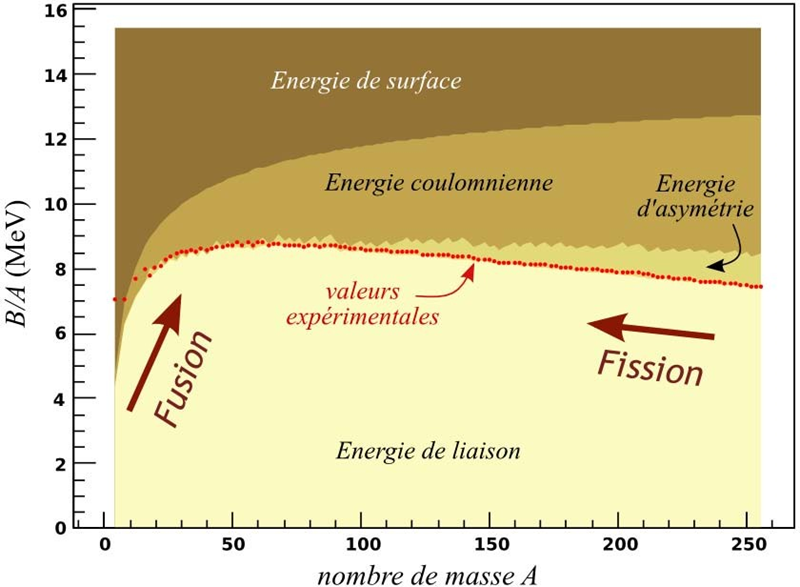
\includegraphics[width=\textwidth]{Chapitre201-img/Chapitre201-img003.png}
 	\caption{Contributions des différents termes dans l'expression de l'énergie de liaison
}
 \end{figure}

\textbf{1.4.2.2 Modèle en couches sphériques}

Le modèle en couches a pour objectif de décrire la structure des noyaux connus ainsi que de prédire celle des noyaux non
encore étudiés. Donc, en première instance, le modèle en couches doit permettre de retrouver ces nombres magiques
établis pour des\textbf{ }noyaux stables. Le modèle en couches décrit des particules indépendantes se déplaçant dans un
potentiel moyen engendré par l'ensemble des nucléons. En première approximation, les particules se déplacent librement,
sans aucune interaction entre elles. Nous nous trouvons donc confronté à la résolution d'un problème à 1 corps où
chaque particule obéit à l'équation de Schrödinger. Dans le cas du modèle en couches sphériques, l'hamiltonien est
constitué d'un potentiel harmonique, donc central. Le choix classique de potentiel moyen central est celui de
l'oscillateur harmonique isotrope, invariant par rotation : ${}$
 \begin{equation}U\left(r\right)=-U_0+\frac 1 2\mu \omega
^2r^2\end{equation} (1.6)
où \textit{U}\textsubscript{0} est la profondeur du puits, $\mu $ la masse réduite du nucléon : $\mu =m\frac{A-1} A$\ ,
m étant la masse du nucléon libre et r la distance entre le nucléon et l'origine du référentiel, $\omega $ est la
fréquence de l'oscillateur harmonique. En raison de la symétrie sphérique, la fonction d'onde d'un nucléon peut être
réécrite en séparant les parties angulaire et radiale comme suit :
\begin{equation}\psi \left(r,\theta ,\varphi
\right)=R_{\mathit{nl}}(r)Y_{\mathit{lm}}(\theta ,\varphi
)
\end{equation}

où \textit{R}\textit{\textsubscript{nl}}\textit{(r)} est la fonction radiale et Y\textit{\textsubscript{lm }}($\theta $, $\varphi $) sont les fonctions harmoniques sphériques, \textit{n} étant le nombre quantique principal et l et m sont
respectivement le moment angulaire orbital et sa projection sur l'axe de quantification. Les valeurs propres, ou les
énergies des états, sont données par :
 \begin{equation}
E_{\mathit{nl}}=(2n+l-\frac 1 2 )\hbar \omega =(N+\frac 3 2) \hbar \omega
\end{equation}
avec N = 2(n$-$1) +l le nombre de quanta excités de l'oscillateur harmonique. \textit{l} prend de valeurs de 0 à N. La
notation spectroscopique fait correspondre aux valeurs de \textit{l} = 0, 1, 2, 3,4, 5, 6 ... les lettres : \textit{s,
p, d, f, g, h, i} ... . Différentes valeurs de \textit{n} et de \textit{l} peuvent conduire à une valeur identique de N
; ces états sont donc dégénérés en énergie, ce qui conduit à la situation se trouvant à l'extrême gauche sur la figure
(1.4 (a)) caractérisée par les nombres quantiques \textit{n} (nombre de phonons de l'oscillateur). La dégénérescence
correspond au nombre de nucléons que peut contenir la couche considérée : \textit{g = }2(2\textit{l+}1). Avec cette
formule, le nombre de nucléons dans un noyau avec couches remplies est 2, 8, 20, 40, 70, 112, . . . On trouve donc les
trois premiers nombres magiques mais pas plus. Un potentiel un peu plus compliqué et plus réaliste que celui de
l'oscillateur harmonique qui tend vers l'infini, est le potentiel de Woods-Saxon. Il modélise la forme aplatie du fond
du puits de potentiel et ainsi reproduit mieux la forme du noyau. Il est paramétrisé par :
\begin{equation} U\left(r\right)=\frac{-U_0}{1+e^{\frac{r-R_0}
a}}\end{equation}
où \textit{r} est la distance radiale du potentiel, \textit{a} est un paramètre de diffusivité et
\textit{R}\textsubscript{0} est le rayon dans lequel $U\left(R\right)=-U_0/2$où \textit{U}\textsubscript{0} définit
la profondeur du puits de potentiel. Les valeurs typiques de ces paramètres sont $U_0\ -50$ MeV, $R_0=r_0A^{1/3}$ et
a${\sim}$0.7 fm.
L'utilisation de ce potentiel comme potentiel moyen ressenti par chaque nucléon permet de lever la dégénérescence en
\textit{l} ; les états de plus grande valeur de \textit{l} étant plus liés, ils sont plus bas en énergie (voir figure
1.4(b)). Considérer un potentiel de Woods-Saxon est équivalent à ajouter au potentiel de l'oscillateur harmonique un
terme en \textit{l}\textsuperscript{2}.
\ Même en utilisant un potentiel plus proche de la réalité, tel que le potentiel de Woods-Saxon, les nombres magiques ne
sont pas reproduits, sauf les 3 premiers (\textbf{2, 8, 20}). Il était assez clair qu'un potentiel central n'arrive pas
à lui seul à reproduire tous les nombres magiques.
 C'est pourquoi, en 1948, M. G. Mayer et, indépendamment, D. Haxel, J. Jensen et H. Suess, ont adjoint au
potentiel de Woods-Saxon, un potentiel dit de spin-orbite \textit{U}\textsubscript{so}, reflétant l'existence d'un
couplage entre le moment angulaire orbital $\overrightarrow l$ et le spin $\overrightarrow s$du nucléon :
\begin{equation} U_0=f(r)\overrightarrow l\overrightarrow
s\end{equation}

 \begin{figure}[htb]
 	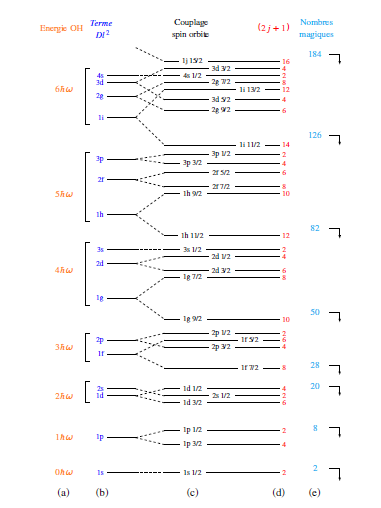
\includegraphics[width=\textwidth]{Chapitre201-img/Chapitre201-img004.png}
 	\caption{(a) Energies des états de particules de l'oscillateur harmonique (O.H.) en fonction de N. (b) Représentation
schématique des énergies des états de particules dans le potentiel de Woods-Saxon, ce qui est équivalent à ajouter au
potentiel O.H un terme en $ l^2$. (c) Représentation schématique de la levée de dégénérescence due au
terme de couplage spin-orbite ; les labels des états sont les nombres quantiques nlj. (d) Nombre de particules
identiques (2\textit{j} + 1) qui peuvent occuper un état. (e) Au niveau des “gap” en énergie, lesnombres magiques sont
reproduits.
}
 \end{figure}

$f(r)$ est la constante de couplage et $\overrightarrow s$est le spin du nucléon et représente son mouvement
intrinsèque. $\overrightarrow l$ et $\overrightarrow s$étant couplés, ils ne sont pas de bons nombres quantiques de
l'hamiltonien. C'est le moment angulaire total $\overrightarrow j=\overrightarrow l$\ + $\overrightarrow s$ qui est un
invariant de H. Le couplage spin-orbite est dû à l'interaction nucléon-nucléon qui ne dépend pas seulement de la
position et du spin des nucléons, mais également de leur vitesse relative. Avec le terme de spin-orbite, les énergies
des états \textit{l} sont séparées pour \textit{j} = l ±1/2, les états de plus grand \textit{j} étant les plus liés
(voir figure 1.4(c)). Le nombre de particules identiques qui peuvent occuper un état quantique, soit la dégénérescence
d'une orbitale (\textit{n l} \textit{j}), est donné par 2 \textit{j} +1 (voir figure1.4(d)). Avec cette modélisation de
l'hamiltonien, la séquence des nombres magiques est alors reproduite (voir figure 1.4(e)). Cependant, ce modèle n'est
valable que pour les noyaux sphériques.

\chapter{La théorie Hartree-Fock-Bogoliubov}

\textcolor{black}{ La théorie Hartree-Fock-Bogoliubov (HFB) est à la fois une extension de la théorie de
Hartree-Fock (HF) et de la théorie de Bardeen-Cooper-Schrieffer (BCS).}\textbf{ }Afin d'avoir une bonne compréhension
de cette approche, il est utile de passer en revue un bref résumé de la théorie la plus générale de Hartree-Fock et de
la théorie de (BCS) de l'appariement.

\section{La théorie Hartree-fock}

 La méthode Hartree-Fock a été introduite par D. Hartree, V. Fock et J. C. Slater pourapproximer l'état
fondamental (et son énergie) de problèmes généraux à N corps en physique quantique. Et la principale application de
cette méthode était, en physique atomique, l'étude des systèmes coulombiens (atomes et molécules) avec l'hamiltonien
purement coulombien des électrons interagissant avec des noyaux statiques. L'approche a été appliquée en physique
nucléaire pour la première fois en 1963 par Kelson.
[Warning: Draw object ignored] La méthode de Hartree-Fock (HF) est basée sur l'hypothèse que les nucléons
composant le noyau peuvent être considérés comme indépendants dans un champ moyen construit de manière auto-cohérente.
Ceci s'explique par la nature quantique des nucléons, le principe de Pauli et la partie fortement répulsive à courte
portée de l'interaction nucléon-nucléon. Ainsi, on peut considérer les nucléons comme des particules indépendantes se
déplaçant dans un potentiel moyen qu'ils créent eux-mêmes.
[Warning: Draw object ignored]
FIG 2.1~Illustration de l'approximation de champ moyen qui consiste à approximer un ensemble de nucléons en interaction
par un ensemble de particules indépendantes dans un champ moyen.
L'ingrédient de base de ces théories est l'hamiltonien microscopique qui régit la dynamique des nucléons individuels
plongés dans un potentiel moyen qu'ils créent collectivement. Cet hamiltonien peut s'écrire sous la forme :
 \begin{equation}H=\sum _{\mathit{ij}}T_{\mathit{ij}}a_i^+a_j+\frac{ 1}{ 4}\sum_{\mathit{ijkl}}V_{\mathit{ijkl}}a_i^+a_j^+a_ka_l
\end{equation}
où le premier terme correspond à l'énergie cinétique et $V_{\mathit{ijkl}}$l'élément de matrice a deux corps de
l'interaction effective. Les opérateurs $a_i^+$ \textit{\ }et $a_i$représentent respectivement les opérateurs
de création et d'annihilation de fermions dans l'état à un corps $|i \rangle$. Ces opérateurs respectant les
règles d'anticommutation,
 \begin{equation}[a_i^+,a_j^+]_+=[a_i,a_j]_+ \mathit{et}[a_i,a_j^+]_+ =[a_i^+,a_j]_+ = \delta_{ij}
\end{equation}
Dans la méthode de \textbf{Hartree-Fock (HF),} La fonction de l'état fondamental du noyau est recherchée sous la forme
d'un déterminant de Slater construit à partir des fonctions d'onde individuelles des nucléons :
\begin{equation}| \left.\Psi _{\mathit{HF}}\right\rangle
=\mathit{det}\left[\Phi _{\mathit{\alpha 1}}\left(x_1\right).\Phi _{\mathit{\alpha 2}}\left(x_2\right){\dots}\Phi
_{\mathit{\alpha A}}\left(x_A\right)\right]\end{equation}
avec $| \left.\Psi _{\mathit{HF}}\right\rangle $la fonction d'onde du noyau. Les équations de Hartree-Fock
s'obtiennent en minimisant l'énergie totale du noyau :
 \begin{equation}E_{\mathit{HF}}=\frac{\left\langle \Psi _{\mathit{HF}}\left|H\left|\Psi _{\mathit{HF}}\right.\right.\right\rangle
}{\left\langle \Psi _{\mathit{HF}}\left|\Psi _{\mathit{HF}}\right.\right\rangle
}\end{equation}
Ce principe variationnel conduit aux équations de Hartree-Fock (HF) \textbf{:}
 \begin{equation}h\Phi _{\beta _i}=\left\{\frac{-\hbar
}{2m}{\nabla}^2+U_{\mathit{HF}}\left[\Phi _{\alpha }\right]\right\}\Phi _{\beta _i}=\varepsilon _{\beta
_i}\end{equation}

\begin{equation} i=1,{\dots},A 
\end{equation}

où le champ Hartree-Fock $U_{\mathit{HF}}\left[\Phi _{\alpha }\right]$ dépend lui-même des fonctions d'onde
individuelles $\Phi _{\alpha }$ générant ainsi un système auto-cohérent de \textit{A }équations
non-linéaires.
Pour résoudre ce système d'équations (Éq. (2.5)), il faudrait déjà connaître la solution ! On procède donc de manière
itérative en postulant une solution (fonction test) et en l'injectant dans le système, ce qui permet de construire le
premier hamiltonien HF que l'on diagonalise. Les états propres et fonctions propres obtenus sont ensuite utilisés pour
reconstruire un nouvel hamiltonien, et ainsi de suite, jusqu'à ce que la variation du jeu de fonctions d'onde entre
deux itérations successives soit inférieure à une valeur fixée. Certaines symétries du système sont généralement prises
en compte lors de la résolution de ces équations : les noyaux pairs-pairs seront par exemple décrits avec un état
$\Psi _{\mathit{HF}}$invariant par renversement du temps (dégénérescence de Kramers) qui permettra de diviser par
deux le nombre d'équations à traiter.
L'approximation de Hartree-Fock est bien adaptée à la description des noyaux pour lesquels il existe, dans le spectre de
particules individuelles un écart en énergie ({\textquotedbl}gap{\textquotedbl}) important entre le dernier niveau
occupé et le premier état vide. Ce {\textquotedbl}gap{\textquotedbl} garantit la stabilité du noyau générant un nombre
magique pour le nombre de neutrons ou de protons correspondant. C'est le cas des noyaux pairs-pairs à couches fermées.
L‘approximation HF est par contre insuffisante dès que l'on veut décrire les états fondamentaux des noyaux situés en
milieu de couches pour lesquels l'état fondamental sera quasiment dégénéré avec une multitude d'autres états obtenus à
partir de configurations de type particule-trou construites sur ce dernier. L'introduction des corrélations
d'appariement permet de restaurer un {\textquotedbl}gap{\textquotedbl} en énergie entre états de
{\textquotedbl}quasi-particules{\textquotedbl}, et ainsi de redonner une bonne solution pour l'état fondamental du
noyau.

\section{Les corrélations d'appariement}

Le concept d'appariement a été introduit en physique de la matière condensée, où, sous l'action d'une interaction
attractive (efficace), les électrons peuvent se coupler pour former les paires de Cooper, responsables à basse
température du phénomène de supraconductivité. Les évidences expérimentales confirmant ce phénomène nucléaire sont
nombreuses et connues depuis longtemps. Résumons brièvement certains de ces faits expérimentaux :

\textbf{Le gap d'énergie}. Les spectres des noyaux déformés montrent une différence caractéristique entre les nombres de
nucléons pairs et impairs. Les noyaux pairs-pairs ne possèdent que quelques niveaux (collectifs) jusqu'à une énergie
d'excitation de 1,5 MeV. La situation est très différente pour les noyaux pairs-impairs, qui ont de nombreux niveaux
collectifs et mono- particulaires dans le même intervalle d'énergie. Figure 2.2 montre le spectre de certains isotopes
de l'étain à titre d'exemple.


 \begin{figure}[htb]
 	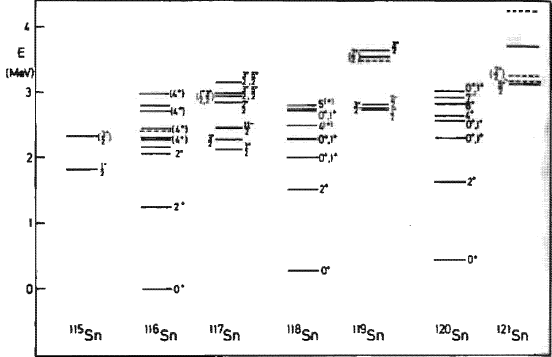
\includegraphics[width=\textwidth]{Chapitre201-img/Chapitre201-img005.png}
 	\caption{ spectre d'excitation des isotopes \textsubscript{50}sn
}
 \end{figure}

Pour les noyaux entre couches fermées, la configuration énergétiquement la plus favorable sera celle dans laquelle tous
les nucléons (sauf le dernier dans le cas des noyaux pairs-impairs) sont appariés. Pour exciter les noyaux
pairs-impairs, nous devons donc briser au moins une paire ce qui demande beaucoup d'énergie contrairement aux noyaux
pairs-impairs dont laquelle une excitation peut être obtenue en plaçant le nucléon impair dans un niveau d'énergie très
bas. L'énergie de liaison d'une paire étant de l'ordre de 1-2 MeV, le gap d'énergie entre l'état fondamental et le
premier état excité dans les noyaux pairs et impairs s'explique donc qualitativement.

\textbf{\ Effet pair-impair}. L'énergie de liaison totale d'un noyau pair-impair est inférieure à la moyenne
arithmétique des énergies de liaison des deux noyaux pairs voisins. Par conséquent, nous avons la relation suivante des
masses des noyaux voisins :
 \begin{equation}M_{\left(A\mathit{impair}\right)}>\frac{M_{A-1}+M_{A+1}}
2\end{equation}
Ce phénomène peut être expliqué par le modèle d'appariement. Lorsque le noyau possède un nombre pair de protons et de
neutrons, chacun de ces nucléons se couple à un autre pour former une pairedans un état de spin opposé afin
d'augmenter la stabilité du noyau.

\textbf{Déformations}. Si, dans le modèle en couche pure, nous calculons la distribution de la densité des nucléons en
fonction du nombre de masse nucléaire. On peut constater que les noyaux à couches fermées ont une forme symétrique
sphérique. Ce n'est pas le cas pour ceux à couchemoitié remplis qui subissent une grande déformation.
L'existence de paires-comme nous l'avons vu dans la fig. (2.2)- favorise une forme nucléaire sphérique (aucune direction
n'est préférable). Les noyaux dont les nombre de massesne dévient pas beaucoup des configurations des couches
fermées auront donc toujours une symétrie sphérique, puisque l'influence de la force d'appariement l'emporte sur la
tendance à la déformation. Plus loin des couches fermées nous aurons la situation inverse. De cette façon, le passage
plutôt soudain de la sphéricité à la déformation peut être compris.

\textbf{Le moment d'inertie} des noyaux déformés peut être mesuré à partir de la structure de niveau des bandes
rotationnelles. Les calculs basés sur le modèle à particule unique pure s'écartent d'un facteur 2 des valeurs
expérimentales. Si l'appariement est inclus, la théorie et l'expérience sont en bien meilleur accord. Donc une
description réaliste des noyaux doit prendre en compte ces corrélations. Ce qui n'est pas le cas dans l'approximation
de Hartree-Fock où l'interaction résiduelle de l'appariement est négligée.

\section{Approximation BCS}
 La méthode {\textquotedbl}'classique{\textquotedbl} de traitement des corrélations d'appariement est
l'approximation BCS, proposée par J. Bardeen, L.N. Cooper et J.R. Schrieffer en 1957. Dans la théorie BCS, la fonction
d'onde de l'état fondamental d'un système pair-pair est approximée par l'expression suivante :
 \begin{equation}| \left.\mathit{BCS}\right\rangle
=\prod _{k>0} (u_k+v_k a_k^+ a_{\overline k}^+  )| \left.0\right\rangle
\end{equation}
où\textit{ k} et $\overline k$ représentent des états appariés à une seule particule et sont reliés par l'opérateur de
renversement du sens de temps, de telle sorte que l'espace des états à un corps est partitionné en des états \textit{k
}{\textgreater} 0 et des états $\overline k$\ {\textless} 0.\textit{u}\textit{\textsubscript{k}} et
\textit{v}\textit{\textsubscript{k}}\textsubscript{ }sont les amplitudes d'occupation
({\textbar}\textit{v}\textit{\textsuperscript{2}}\textit{\textsubscript{k}}{\textbar} est la probabilité que la paire
(\textit{k}, $\overline k$) soit occupée et $\left|\left.u_k^2\right|+\left|v_k^2\right.\right|=1$.
 Le système est donc décrit en terme de paires indépendantes, et non en terme de particules indépendantes.
 Le nombre de particules dans la théorie BCS n'est pas conservé ; il n'est fixé qu'en valeur moyenne par
(en contraignant le système par un multiplicateur de Lagrange $\lambda $) :
\begin{equation}\left\langle
\mathit{BCS}\left|\widehat N\left|\mathit{BCS}\right.\right.\right\rangle =\sum
_{k>0}2v_k^2=N\end{equation}
 Cette violation du nombre de particules n'a pas beaucoup d'importance en physique du solide, où le nombre
de particules est typiquement de l'ordre ou proche du nombre d'Avogadro (N ${\simeq}$ 10\textsuperscript{23}). La
dispersion qu'on peut montrer être égale à $1/{\surd}N$, est donc faible. Ceci n'est pas le cas en physique nucléaire
où N ${\approx}$ 10$-$100 et donc le problème devient réel.
 L'approximation BCS permet donc un traitement approché des effets d'appariement. Cependant, elle brise une
symétrie (celle de la conservation du nombre de particules) qui s'ajoute aux symétries déjà brisées dans
l'approximation d'HF, ce qui est un point de défaut. En plus, cette approche présente l'inconvénient de ne pas être
adaptée pour le cas des noyaux impairs. Il est nécessaire de la généraliser selon la méthode de Hartree Fock
Bogoliubov(HFB).
\section{Concept de quasi-particules}
 Pour tenir compte des effets d'appariement dans le noyau\textbf{,} on introduit le concept de
quasiparticules deBogoliubov dans la méthode hartree-fock. On transforme ainsi l'état HF de particules indépendantes
 ${a,a^+}$ en un état Hartree-Fock-Bogoliubov (HFB) de quasi-particules indépendantes ${\beta ,\beta ^+}$en utilisant la transformation suivante :
 \begin{equation}\beta _{\alpha }=\sum
_iU_{\mathit{i\alpha }}^{\ast }a_i+V_{\mathit{i\alpha }}^{\ast
}a_i^+
\end{equation}

\begin{equation}
\beta _{\alpha }^+=\sum
_iU_{\mathit{i\alpha }}a_i^++V_{\mathit{i\alpha
}}a_i
\end{equation}
Les équations (6,7) peuvent être écrites sous forme matricielle :

 \begin{equation}
(\beta \beta^+  )=(U^+  V^+ V^T U^T ) (a a^+) = W^+ (a a^+ )
\end{equation}


La transformation de Bogoliubov préserve les relations d'anticommutation. Le calcul des anticommutateurs entre les
opérateurs de création\textit{ $\beta $}\textsuperscript{†}\textit{\textsubscript{i}} et d'annihilation \textit{$\beta
$}\textsubscript{j} de quasi-particules permet de montrer que la matrice $W$\ (matrice de Bogoliubov) est unitaire :
$WW^+=W^+W=1$ 
c'est à dire :
 \begin{equation}U^+U+V^+V=1\end{equation} ,
 \begin{equation}UU^++V^{\ast }V^T=1\end{equation}
 \begin{equation}U^TV+V^TU=0\end{equation} ,
$UV^{\ast }+V^{\ast }U^T=0$

\section{La méthode Hartree fock-bogoliubov}

 Dans l'approximation HFB, l'hamiltonien est essentiellement réduit à deux potentiels : le potentiel moyen
auto-cohérent \textcolor[rgb]{0.1254902,0.12941177,0.13333334}{$\Gamma $} de la théorie de Hartree-Fock, et un champ
d'appariement supplémentaire $\Delta $, connu de la théorie BCS.
 L'état HFB, noté $ | \Phi \rangle $, est défini comme le vide associé aux opérateurs d'annihilation de
quasi-particules \textit{$\beta $}\textit{\textsubscript{i}}. Il vérifie donc, pour tout \textit{i} :
 \begin{equation} \beta _i| \left.\Phi \right\rangle =0 \end{equation}
On impose de plus à cet état d'être normé :
 \begin{equation} \left\langle \Phi \left|\Phi \right.\right\rangle
=0\end{equation}
L'hamiltonien nucléaire H, qui décrit le système de Z+N = A nucléons, contient un terme cinétique T à un corps et une
série de termes V\textsuperscript{(n)} qui décrivent les interactions simultanées de n nucléons entre eux :
 \begin{equation}H=T+V^{\left(2\right)}+V^{\left(3\right)}+{\dots}V^{\left(A\right)}\end{equation}

Le terme cinétique \textit{T} décrit un système de A particules libres. Le terme à deux corps décrit l'interaction entre
chaque paire de particules :
 \begin{equation}
V^{\left(2\right)}=\frac 1 2\sum
_{i{\neq}j=1}^Av_{\mathit{ij}}\end{equation}

où l'opérateur \textit{v}\textsubscript{ij }décrit l'interaction à deux corps entre la particule \textit{i} et la
particule \textit{j}. Les termes décrivant les interactions à trois corps ou plus seront négligés. L'hamiltonien
nucléaire H se réécrit :
 \begin{equation}H=\sum
_{i=1}^At_{\mathit{ij}}+\frac 1 2\sum
_{i{\neq}j=1}^Av_{\mathit{ij}}\end{equation}

et en seconde quantification :
\begin{equation}H=\sum _{\mathit{ij}}T_{\mathit{ij}}a_i^+a_j+\frac{1}{4} \sum_{\mathit{ijkl}}V_{\mathit{ijkl}}a_i^+a_j^+a_k a_l\end{equation}

avec \textit{v}\textit{\textsubscript{ijk}}, les éléments de matrice de l'interaction NN antisymétrisée :
\begin{equation}V_{\mathit{ijkl}}=\left\langle \mathit{ij}\left|v\left|\mathit{kl}\right.\right.\right\rangle -\left\langle
\mathit{ij}\left|v\left|\mathit{lk}\right.\right.\right\rangle
\end{equation} 

Pour un état HFB $ | \Phi \rangle $ donné, l'énergie moyenne E\textsubscript{HFB} de cette configuration sera
donnée~par :

 \begin{equation}E_{\mathit{HFB}}=\left\langle \Phi \left|H\left|\Phi \right.\right.\right\rangle =\sum
_{\mathit{ij}}t_{\mathit{ij}}\rho _{\mathit{ij}}+\frac 1 2\sum _{\mathit{ijkl}}v_{\mathit{ijkl}}\left[\rho
_{\mathit{ki}}\rho _{\mathit{lj}}+\frac 1 2k_{\mathit{ij}}^{\ast }k_{\mathit{kl}}\right]\end{equation} 

où $\rho $ est la matrice densité du système, définie par :
 \begin{equation}
\rho = \langle \Phi \rangle  =\sum _m V_i^{m\ast
}V_j^m
\end{equation}

La densité $\rho $ est une observable, elle est donc hermitienne, soit : $\rho $† = $\rho $. La trace de la matrice
densité correspond au nombre total de particules qu'il contient :
 \begin{equation} N=\mathit{tr}\left(\rho \right)=\sum _{\Im }V_i^{m\ast
}V_i^m\end{equation} 

La norme du vecteur V\textit{\textsubscript{i}} donne la contribution des quasi-particules au nombre total de particules
N dans le système. Lorsque {\textbar}V\textit{\textsubscript{i}}{\textbar}\textsuperscript{2} {\textgreater} 1/2, c'est
un état de trou et lorsque {\textbar}V\textit{\textsubscript{i}}{\textbar}\textsuperscript{2} {\textless} 1/2c'est un
état de particule, en moyenne.

Le terme \textit{K} est le tenseur d'appariement (ou densité anormale) définie par :
 \begin{equation}K_{\mathit{ij}}=\langle \Phi \rangle =\sum _mV_i^{m\ast}U_j^m
\end{equation}

\textcolor{black}{Le terme en }\textit{\textcolor{black}{K*K}}\textcolor{black}{, dans l'équation de l'énergie
}\textit{\textcolor{black}{E}}\textit{\textcolor{black}{\textsubscript{HFB}}}\textcolor{black}{, représente la
contribution des corrélations d'appariement à l'énergie. Dans la limite où l'appariement est nul, on retrouve l'énergie
moyenne de la théorie HF.}
Il est également utile de définir la matrice densité généralisée, notée R, qui permet de regrouper la matrice densité a
un corps, $\rho $, et le tenseur d'appariement, k, en une seule matrice. Elle est définie comme :
 \begin{equation}R=\left(\begin{matrix}\rho
&k\\-k^{\ast }&1-\rho ^{\ast
}\end{matrix}\right)\end{equation}
et dont les vecteurs propres sont les coefficients $\left(\genfrac{}{}{0pt}{0}{u_i}{v_i}\right)$ définissant la
transformation unitaire de Bogoliubov.
\textcolor{black}{ On minimise l'énergie EHFB de la même manière que pour HF, en utilisant un principe
variationnel. On obtient alors les équations HFB qui s'écrivent sous forme matricielle :}
\textcolor{black}{}

 \begin{equation} H_{\mathit{HFB}}=\left(\genfrac{}{}{0pt}{0}{u_i}{v_i}\right)=\left(\begin{matrix}h&{\Delta}\\-{\Delta}^{\ast
}&-h^{\ast
}\end{matrix}\right)\left(\genfrac{}{}{0pt}{0}{u_i}{v_i}\right)=E_i\left(\genfrac{}{}{0pt}{0}{u_i}{v_i}\right)\end{equation}

 \begin{equation}H_{\mathit{HFB}}=\left(\genfrac{}{}{0pt}{0}{u_i^{\ast }}{v_i^{\ast
}}\right)=\left(\begin{matrix}h&{\Delta}\\-{\Delta}^{\ast }&-h^{\ast
}\end{matrix}\right)\left(\genfrac{}{}{0pt}{0}{u_i^{\ast }}{v_i^{\ast }}\right)=E_i\left(\genfrac{}{}{0pt}{0}{u_i^{\ast
}}{v_i^{\ast }}\right)
\end{equation}

où h est le champ particule-trou (champ Hartree-Fock) :

 \begin{equation}h_{\mathit{ik}}=\frac{\delta (E-\lambda _pZ-\lambda _nN)}{\delta \rho _{\mathit{ki}}}=h_{\mathit{ki}}^{\ast
}\end{equation}

et $\Delta $ est le champ d'appariement dont les éléments de matrices sont :


 \begin{equation}{\Delta}_{\mathit{ij}}=\frac{\delta (E-\lambda _pZ-\lambda _nN)}{\delta k_{\mathit{ji}}^{\ast
}}={\Delta}_{\mathit{ji}}^{\ast }
\end{equation}

$\lambda $p et $\lambda $n sont les multiplicateurs de Lagrange correspondant respectivement aux
potentiels chimiques des protons et neutrons :

 \begin{equation}
\lambda _p=\frac{\mathit{\delta E}}{\mathit{\delta Z}}, \lambda _n=\frac{\mathit{\delta E}}{\mathit{\delta N}}
\end{equation}

\textcolor{black}{ce qui donne pour une force à deux corps ne dépendant pas de la densité, d'après la définition}
\textcolor{black}{de l'Hamiltonien nucléaire (Eq. 2.19) :}

 \begin{equation}h_{\mathit{ik}}=t_{\mathit{ik}}+\sum _{\mathit{jl}}v_{\mathit{ijkl}}\rho
_{\mathit{lj}}
\end{equation}

\textcolor{black}{et}\textcolor{black}{
\ }

 \begin{equation}
 {\Delta}_{\mathit{ik}}=\frac 1 2\sum
_{\mathit{kl}}v_{\mathit{ijkl}}K_{\mathit{kl}}
\end{equation}

\textcolor{black}{ Pour conclure, la théorie HFB permet, grâce à la prise en compte des corrélations d'appariement,
d'améliorer la fonction d'onde approchant l'état fondamental dans les noyaux non magiques, et ceci en régénérant un gap
au-dessus du niveau de Fermi similaire à celui observé dans les noyaux magiques à l'approximation HF à travers une
transformation de Bogoliubov.}


 \begin{figure}[htb]
 	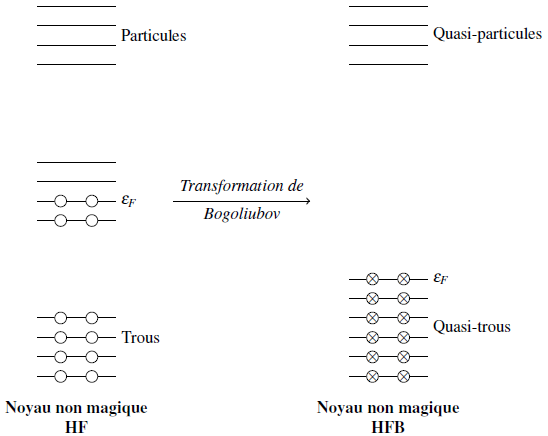
\includegraphics[width=\textwidth]{Chapitre201-img/Chapitre201-img006.png}
 	\caption{Représentation schématique du spectre d'un noyau non magique traité avec la théorie HF (gauche) et avec HFB
(droite). Un gap entre les états de quasi-trous et quasi-particules est généré via la transformation~de Bogoliubov.
}
 \end{figure}

\section{Les interactions Effectives phénoménologiques}

Dans la pratique, la méthode HFB demande une interaction effective pour calculer le champ
d'appariement $\Delta $ et le champ Hartree-Fock (HF) h.\textbf{\textcolor{black}{ }}Plusieurs interactions effectives
phénoménologiques ont été développées ces dernières années. Ce type d'interaction est représenté sous une forme
analytique paramétrisable puis ajuste sur des propriétés générales du milieu nucléaire. Les paramètres sont alors
définis une fois pour toutes. Les deux grandes familles de forces utilisées actuellement sont
:\textbf{\textcolor{black}{ }}
\begin{itemize}
\item \textbf{Interactions de portée finie}
\end{itemize}
 À partir des années 60 et jusqu'à nos jours, l'interaction effective de portée finie est probablement la
plus étudiée parce que peut-être la plus naturelle. La portée finie permet en effet une meilleure simulation des longue
et moyenne portées de l'interaction nucléon-nucléon(NN) réaliste. Elle autorise en outre un traitement auto-cohérent
des corrélations d'appariement dans un formalisme Hartree-Fock-Bogoliubov (HFB) : dans l'espace des moments la portée
des corrélations d'appariement sera finie éliminant ainsi toute divergence. C'est à l'évidence un atout important dès
que l'on veut s'éloigner vers les grandes déformations ou vers les lignes d'instabilité proton ou neutron, les
corrélations d'appariement s'adaptant automatiquement à ces nouvelles conditions.
 La force de Gogny est modélisée par une somme de termes gaussiens attractifs ou répulsifs, A ces éléments,
il faut ajouter un terme dépendant de la densité ainsi qu'un terme d'interaction spin-orbite, tous deux de portée
nulle. Son expression générale en représentation coordonnée s'écrit :
\begin{equation*}
V\left(\overrightarrow r_1,\overrightarrow r_2\right)=\sum _{i=1}^2\left[W_i+B_iP_{\sigma }-H_iP_{\tau }-M_iP_{\sigma
}P_{\tau }\right]e^{\frac{-r^2}{\mu _i}}+t_3\left(1+x_3P_{\sigma }\right)[\rho (\overrightarrow R)]_{\alpha }\delta
\left(\overrightarrow r\right)
\end{equation*}
\begin{equation}+iW_0\overrightarrow{\sigma }.\left[\overrightarrow P\ast {\wedge}\delta
\left(\overrightarrow r\right)\overrightarrow P\right]\end{equation}
\begin{itemize}
\item \textbf{Interaction de portée nulle : la force de Skyrme}
\end{itemize}
\textcolor[rgb]{0.13725491,0.12156863,0.1254902}{ La force de Skyrme est une interaction effective
phénoménologique de portée nulle qui permet de modéliser de façon simple les interactions entre les nucléons dans le
noyau. Proposée en 1956 par T.H.R, Skyrme. }La portée nulle permet de simplifier les calculs numériques. Ces forces
sont représentées, mathématiquement, par une \textcolor{black}{distribution de Dirac $\delta $(} $\overrightarrow
r$\textcolor{black}{):}
\begin{equation*}
V\left(\overrightarrow{r_1},\overrightarrow{r_2}\right)=t_0(1+x_0P_{\sigma })\delta (\overrightarrow r)
\end{equation*}
 \begin{equation}+t_2\left(1+x_2P_{\sigma }\right)\overrightarrow{P^{\ast }}\delta \left(\overrightarrow
r\right)\overrightarrow P+\frac 1 6t_3(1+x_3P_{\sigma })[\rho (\overrightarrow R)]^{\alpha }\delta
\left(\overrightarrow r\right)\end{equation}
\begin{equation*}
+iw_0\overrightarrow{\sigma }.[\overrightarrow{P^{\ast }}{\wedge}\delta \left(\overrightarrow r\right)\overrightarrow P]
\end{equation*}
avec les notations usuelles :
\begin{equation}r=r_1-r_2\end{equation} , \begin{equation}R=\frac 1 2(r_1+r_2)\end{equation}

\begin{equation}P=\frac 1{2i}({\nabla}_1-{\nabla}_2)P^{\ast } \end{equation} 
cc de $\overrightarrow P$agissant à gauche et également

 \begin{equation}\sigma =\sigma _1+\sigma _2\end{equation} ; \begin{equation}P_{\sigma
}=(1+\sigma _1.\sigma _2)/2\end{equation}
\textcolor[rgb]{0.13725491,0.12156863,0.1254902}{ Au premier terme, terme central décrivant le terme
attractif de la force, il convient d'ajouter deux termes « non locaux », Ceux-ci, qui dépendent des vitesses, peuvent
être vus}\textit{\textcolor[rgb]{0.13725491,0.12156863,0.1254902}{
}}\textcolor[rgb]{0.13725491,0.12156863,0.1254902}{comme une simulation de portée nulle d'effets de portée finie comme
introduits dans la force de Gogny. Le dernier terme est un terme d'interaction spin-orbite indispensable pour
reproduire la série des nombres magiques dans les noyaux qui, comme nous l'avons déjà mentionné auparavant, est
construit de manière purement phénoménologique.}




\chapter{Propriétés de l’état fondamental des isotopes pairs et impairs de Fl, Lv  et Og}


\section{Résumé}

\textbf{ }Afin d'étudier les propriétés de l'état fondamental\textbf{ }des isotopes pairs et impairs  de\textcolor[rgb]{0.1254902,0.12941177,0.13333334}{~Flérovium} (Fl, Z=114),\textbf{\textcolor[rgb]{0.1254902,0.12941177,0.13333334}{ }}\textcolor[rgb]{0.1254902,0.12941177,0.13333334}{Livermorium }(Lv, Z=116) et L’oganesson (Og, Z=118), la matrice HFB est résolue en utilisant le code HFBTHO version 3.00 [14], avec l'interaction Skyrme SLy4, où l’ensemble de paramètres typiques de cette force est présentés dans le tableau (3.1). 

Dans ce chapitre, nous avons présenté les résultats numériques de notre étude y compris l'énergie de liaison, l'énergie de séparation des deux neutrons, les rayons de charge, de neutrons et de protons. L’énergie d’appariement et le spectre d’énergie. Les résultats ont été comparés avec les données expérimentales disponibles et avec les prédictions de certains modèles nucléaires tels que le modèle de la gouttelette liquide à portée finie (Finite Range Droplet Model, FRDM) et la théorie du champ moyen relativiste (RMF).

\section{Code HFBTHO v 3.00} \textbf{ }

\section{Détails des calculs}


 Dans le présent travail, Les calculs ont été effectués avec le code HFBTHO v3.00 [14] et ont été exécutés de manière répétitive avec un script python pour modifier les entrées et pour enregistrer et analyser les données de sortie. Parmi plusieurs ensembles de paramètres pour la prédiction des propriétés de l’état fondamental nucléaire, nous avons utilisé la force de Skyrme SLy4 [15] qui est largement utilisée dans les calculs de la structure nucléaire. La force de Skyrme SLy4 a été développée par E. Chabanat et ses collaborateurs. Elle fait partie de la famille de forces SLyx. Pour déterminer l’ensemble des paramètres de cette force (10 au total), les auteurs ont suivi un protocole d’ajustement incluant certaines propriétés de la matière nucléaire infinie (valeur de saturation ρ\textsubscript{0} et coefficient d’incompressibilité) et quelques propriétés de la matière nucléaire finie (masses et rayons de quelques noyaux doublement magiques). Cette force a été construite pour des conditions extrêmes d’isospin et de densité. Néanmoins, elle conduit à de très bons résultats pour les noyaux de la vallée de stabilité et les noyaux fortement déformés.

 L’ensemble des paramètres SLy4 [15] utilisés dans cette étude est présenté dans le tableau 3.1.

 \textbf{ Table 3.1 }Paramètres de la force de Skyrme SLy4

\begin{center}
\tablefirsthead{}
\tablehead{}
\tabletail{}
\tablelasttail{}
\begin{supertabular}{m{1.8900598in}m{1.8893598in}}
\hline
\centering{\begin{english}\bfseries\color{black} Parameter\end{english}} &
\centering\arraybslash{\begin{english}\bfseries\color{black} Sly4\end{english}}\\\hline
\centering{\color{black}  $t_0$\textenglish{ (MeV fm}\textenglish{\textsuperscript{3}}\textenglish{)}} &
\centering\arraybslash{\begin{french}\color{black} -2484.91\end{french}}\\
\centering{\color{black}  $t_1$\textenglish{ (MeV fm}\textenglish{\textsuperscript{5}}\textenglish{)}} &
\centering\arraybslash{\begin{french}\color{black} 486.82\end{french}}\\
\centering{\color{black}  $t_2$\textenglish{ (MeV fm}\textenglish{\textsuperscript{5}}\textenglish{)}} &
\centering\arraybslash{\color{black} -546.39}\\
\centering{\color{black}  $t_3$\textenglish{ (MeV fm}\textenglish{\textsuperscript{4}}\textenglish{)}} &
\centering\arraybslash{\color{black} 13777.0}\\
\centering  $x_0$ &
\centering\arraybslash{\color{black} 0.834}\\
\centering  $x_1$ &
\centering\arraybslash{\color{black} -0.344}\\
\centering  $x_2$ &
\centering\arraybslash{\begin{french}\color{black} -1.0\end{french}}\\
\centering  $x_3$ &
\centering\arraybslash{\begin{english}\color{black} 1.354\end{english}}\\
\centering{\color{black}  $W_0$\textenglish{ (MeV fm}\textenglish{\textsuperscript{5}}\textenglish{)}} &
\centering\arraybslash{\color{black} 123}\\
\centering  $σ$ &
\centering\arraybslash{\begin{french}\color{black} 1/6\end{french}}\\\hline
\end{supertabular}
\end{center}

nous avons modifié les valeurs de la force d'appariement pour les neutrons  $V_{n0}$ et protons  $V_{p0}$ (en MeV), qui peuvent être différentes, mais dans notre étude, la force d'appariement  $V_{n,p0}$  est considérée comme étant la même pour les deux. Pour chaque isotope, nous avons exécuté le code en utilisant un  $V_{n,p0}$  et  nous avons comparé l'énergie de liaison totale obtenue à l'état fondamental obtenue avec la valeur expérimentale. Cette procédure a été répétée jusqu'à ce que nous trouvions, pour chaque nombre de masse A (pair et impair), la valeur de  $V_{n,p0}$  qui donne l'énergie de liaison totale à l'état fondamental la plus proche de la valeur expérimentale.

 L’ensemble des résultats numérique des paramètres calculés en utilisant le code HFBTHO version 3.00  est regroupé dans le tableau ci-dessous :




\begin{flushleft}
\tablefirsthead{}
\tablehead{}
\tabletail{}
\tablelasttail{}
\begin{supertabular}{|m{5.78026in}|}
\hline
{\begin{french} \textbf{  Table 3.2 }L'énergie de liaison, l'énergie de séparation d’un et des deux neutrons, les rayons de charge, de neutrons et de protons et L’énergie d’appariement des isotopes de Fl,Lv,Og\end{french}}

{\bfseries  \textenglish{The big table a smail}}\\\hline
\end{supertabular}
\end{flushleft}
\section{ Énergie de liaison}

 L'énergie de liaison est importante dans l'étude de la physique nucléaire et a une relation directe avec la stabilité des noyaux. L'énergie de liaison nucléaire est définie comme l'énergie qui doit être fournie pour briser le noyau d'un atome en protons et neutrons séparés. Dans cette étude, nous calculons l'énergie de liaison moyenne par nucléon (𝐵𝐸⁄𝐴) d'un état fondamental pour les isotopes pairs et impairs de Fl, Lv et Og  dont les résultats sont dressées dans le tableau 3.2 et tracées dans la figure 3.1. Pour montrer la validité de nos calculs, nous les comparons avec les données expérimentales disponibles [16], FRDM(2012) [17] et RMF[18].

\begin{flushleft}
\tablefirsthead{}
\tablehead{}
\tabletail{}
\tablelasttail{}
\begin{supertabular}{|m{6.27126in}|}
\hline
{\begin{french}\bfseries  LES GRAPHES POUR  Fl, Lv, Og\end{french}}

{\begin{french} FIG 3.1 Energies de liaison par nucléon pour les isotopes pairs et impairs de Fl, Lv et d’Og (en MeV).\end{french}}\\\hline
\end{supertabular}
\end{flushleft}
 A partir de la figure 3.1, on voit que les énergies de liaison par nucléon des isotopes de Fl, Lv et d’Og produites par nos calculs en utilisant HFB avec les paramètres SLy4 sont en bon accord avec les données expérimentales. Nous notons aussi que le maximum d’énergie de liaison par nucléon (BE/A), pour les isotopes de  Fl, est observé en n=184 qui pourrait être le 8ème nombre magique.

 Les erreurs maximales approximatives des énergies de liaison par nucléon (BE/A) entre les résultats théoriques et les données expérimentales pour Fl, Lv et Og sont listées dans le tableau 3.3.

 \textenglish{\textbf{TABLE 3.3}}\textenglish{ L’erreur maximale (BE/A)theor −(BE/A)exp (en Mev).}

\begin{center}
\tablefirsthead{}
\tablehead{}
\tabletail{}
\tablelasttail{}
\begin{supertabular}{m{1.2004598in}m{1.2004598in}m{1.2011598in}m{1.2004598in}}
\hline
{\begin{french}\color{black} nayou\end{french}} &
{\begin{french}\color{black} ce travail\end{french}} &
{\begin{french}\color{black} FRDM\end{french}} &
{\begin{french}\color{black} RMF\end{french}}\\\hline
{\begin{french}\bfseries\color{black} Fl\end{french}} &
{\begin{french}\color{black} 0.00336\end{french}} &
{\begin{french}\color{black} 0.02212\end{french}} &
{\begin{french}\color{black} 0.02542\end{french}}\\
{\begin{french}\bfseries\color{black} Lv\end{french}} &
{\begin{french}\color{black} 0.00665\end{french}} &
{\begin{french}\color{black} 0.01555\end{french}} &
{\begin{french}\color{black} 0.01903\end{french}}\\
{\begin{french}\bfseries\color{black} Og\end{french}} &
{\begin{french}\color{black} 0.00895\end{french}} &
{\begin{french}\color{black} 0.01474\end{french}} &
{\begin{french}\color{black} 0.01209\end{french}}\\\hline
\end{supertabular}
\end{center}
\section{Énergie de séparation de neutrons}

 Les énergies de séparation d’un neutron et de deux neutrons sont des quantités très importantes dans l’étude de la structure nucléaire. Dans ce travail, nous les avons calculées pour les isotopes pairs et impairs de Fl, Lv et Og dans la paramétrisation SLy.

L’énergie de séparation d’un neutron, Sn, est définie comme suit :

   \begin{equation}S_n\left(Z,N\right)=\mathit{BE}\left(Z,N\right)-\mathit{BE}(Z,N-1)\end{equation} 

et l’énergies de séparation de deux neutrons, S\textsubscript{2n}, est donnée par :

\begin{equation}S_{2n}\left(Z,N\right)=\mathit{BE}\left(Z,N\right)-\mathit{BE}(Z,N-2)\end{equation} 

Les énergies \textit{S}\textit{\textsubscript{n}}\textit{ }et \textit{S}\textit{\textsubscript{2n}} calculées pour les isotopes de Fl, Lv et  Og sont affichées sur les figures 3.2 et 3.3, respectivement. Les données expérimentales disponibles [16], les prédictions des modèles FRDM [17] et RMF [18] sont aussi présentés à titre de comparaison.

\begin{flushleft}
\tablefirsthead{}
\tablehead{}
\tabletail{}
\tablelasttail{}
\begin{supertabular}{|m{6.31846in}|}
\hline
{\begin{french}  FIG 3.2 Les énergies de séparation d’un neutron,  $S_n$, des isotopes de Fl ,Lv et Og.\end{french}}\\\hline
\end{supertabular}
\end{flushleft}
\begin{flushleft}
\tablefirsthead{}
\tablehead{}
\tabletail{}
\tablelasttail{}
\begin{supertabular}{|m{6.31846in}|}
\hline
{\begin{french} FIG 3.3 Les énergies de séparation de deux neutrons,  $S_{2n}$, des isotopes de Fl, Lv de Og.\end{french}}\\\hline
\end{supertabular}
\end{flushleft}
 D’après les figures 3.2 et 3.3, on voit clairement que les énergies de séparation expérimentales sont bien reproduites par nos calculs. Malgré les légères différences dans le cas de certains isotopes, nos résultats ont l’erreur moyenne absolue la plus faible par rapport aux autres modèles, comme nous pouvons le voir dans le tableau 3.4.

\textbf{TABLE 3.4} L’erreur absolue moyenne (S\textit{\textsubscript{2n}})theor −(S\textit{\textsubscript{2n}})exp et (S\textit{\textsubscript{n}})theor −(S\textit{\textsubscript{n}})exp (en Mev).

\begin{center}
\tablefirsthead{}
\tablehead{}
\tabletail{}
\tablelasttail{}
\begin{supertabular}{|m{0.84275985in}|m{0.8420598in}|m{0.84275985in}|m{0.84275985in}|m{0.84275985in}|m{0.84275985in}|m{0.8420598in}|}
\hline
 &
\multicolumn{3}{m{2.6850598in}|}{\centering  $(S?_{2n})_{\mathit{theor}}-(S?_{2n})_{\exp }$} &
\multicolumn{3}{m{2.68506in}|}{\centering  $(S?_n)_{\mathit{theor}}-(S?_n)_{\exp }$}\\\hline
 &
{\begin{french} This work\end{french}} &
{\begin{french} FRDM\end{french}} &
{\begin{french} RMF\end{french}} &
{\begin{french} This work\end{french}} &
{\begin{french} FRDM\end{french}} &
{\begin{french} RMF\end{french}}\\\hline
{\begin{french} Fl\end{french}} &
 &
 &
 &
 &
 &
\\\hline
{\begin{french} Lv\end{french}} &
 &
 &
 &
 &
 &
\\\hline
{\begin{french} Og\end{french}} &
 &
 &
 &
 &
 &
\\\hline
\end{supertabular}
\end{center}
\section{Rayons de neutron, de proton et de charge  \ \ }

 Le rayon quadratique moyen de charge (rms), R\textit{\textsubscript{c}}, est liée au rayon du proton, R\textit{\textsubscript{p}}, par

 \begin{equation} R_c^2=R_p^2+0.64(\mathit{fm})\end{equation} 

où le facteur 0.64 dans l’équation (3.3) tient compte des effets de taille finie du proton. Dans la figure 3.4, les rayons de charge quadratique prédits par nos calculs HFB sont comparés avec les données expérimentales disponibles [], les prédictions de la théorie RMF [18] et la théorie FRDM~.Les valeurs numériques des rayons de charge sont présentées dans le tableau 3.2

Un bon accord entre la théorie et l’expérience peut être clairement vu dans la figure 3.4. 

\begin{flushleft}
\tablefirsthead{}
\tablehead{}
\tabletail{}
\tablelasttail{}
\begin{supertabular}{|m{6.40316in}|}
\hline
{\begin{french} FIG 3.4 Les rayons de charge obtenus par nos calculs HFB comparés aux données expérimentales disponibles, les prédictions de la théorie RMF [18] et la théorie FRDM [17].\end{french}}\\\hline
\end{supertabular}
\end{flushleft}
La figure 3.5 montre les rayons de neutrons et de protons des isotopes de Fl, Lv et Og obtenus dans nos calculs. Les prédictions de la théorie de RMF et de la théorie FRDM sont également données à titre de comparaison. Nous  avons tracé les rayons de neutrons et de protons (Rn et Rp) ensemble afin de voir la différence entre eux. Les valeurs numériques des rayons de neutrons et de protons des isotopes de Fl, Lv et Og sont dressées dans le tableau 3.2.

\begin{flushleft}
\tablefirsthead{}
\tablehead{}
\tabletail{}
\tablelasttail{}
\begin{supertabular}{|m{6.22476in}|}
\hline
{\begin{french} FIG~3.5 Les rayons de neutrons et de protons des isotopes de Fl, Lv et Og.\end{french}}

\\\hline
\end{supertabular}
\end{flushleft}
\section{Le gap d’appariement}

 Le gap d’appariement n’est pas directement accessible expérimentalement. Par conséquent, il existe diverses formules de différences finies dans la littérature, qui sont souvent interprétées comme une mesure du gap d’appariement empirique, telles que :

La formule de la différence de trois points [19] :

\begin{equation}∆_N^{\left(3\right)}\left(N\right)=\frac{\mathit{πN}} 2[E_b\left(Z,N-1\right)-2E_b\left(Z,N\right)+E_b\left(Z,N+1\right)]\end{equation} 

où N et Z sont les nombres de neutrons et de protons et \textit{E}\textit{\textsubscript{b}} est l’énergie de liaison (négative) du noyau.  $π_N=(-1)^N$  est le nombre de parité.

 Une autre relation couramment utilisée est la formule de la différence de quatre points [20] :

 \begin{equation}∆_N^{\left(4\right)}\left(N\right)=\frac{\mathit{πN}} 4[E_b\left(Z,N-2\right)-3E_b\left(Z,N-1\right)+3E_b\left(Z,N\right)-E_b\left(Z,N+1\right)]\end{equation} 

 Dans la figure 3.6, les gaps d’appariement des neutrons obtenus dans nos calculs HFB sont comparés aux données expérimentales obtenu à partir des énergies de liaison données de la Référence [16] en utilisant les formules de trois points Δ\textsuperscript{(3)}, de quatre points Δ\textsuperscript{(4)} et avec les prédictions du model FRDM [17]. 

\begin{flushleft}
\tablefirsthead{}
\tablehead{}
\tabletail{}
\tablelasttail{}
\begin{supertabular}{|m{6.4018598in}|}
\hline
{\begin{french}  FIG 3.6 Les gaps d’appariement des isotopes de Fl, Lv et Og.\end{french}}\\\hline
\end{supertabular}
\end{flushleft}

\section{L’énergie d’appariement}

\textbf{ A suivre~………………………}

\section{Conclusion}

La théorie HFB avec la force de Skyrme SLy4 a été utilisée pour étudier les propriétés de l’état fondamental de chaînes isotopiques paires et impaires de Fl, Lv et Og. Les énergies de liaison, les énergies de séparation de deux neutrons, et les rayons de charge, de protons et de neutrons ont été calculés ainsi que le gap d’appariement. Les résultats de ces calculs reproduisent très bien les données expérimentales disponibles, y compris l’énergie de liaison par nucléon, les énergies de séparation d’un et de deux neutrons, les rayons de neutrons, de protons, et de charge, le gap d’appariement des neutrons. 



\section[Bibliography]{\textenglish{Bibliography}}
\textenglish{[1 ] El Bassem, Younes, and Mustapha Oulne. "Nuclear structure investigation of even–even and odd Pb isotopes by using the Hartree–Fock–Bogoliubov method." International Journal of Modern Physics E 26.12 (2017): 1750084.}

\textenglish{[2] Balbuena, Edgar Teran. Hartree-Fock-Bogoliubov calculations for nuclei far from stability. Vanderbilt University, 2003.}

\textenglish{[3] G. Audi and A.H. Wapstra, Nuclear Physics A565, 1 (1993).}

\textenglish{[4] JOLIOT-CURIE, E. I., BLAIZOT, J., POES, A., HEENEN, P., VAN DUPPEN, P., GALL, B., ... }\& HELLO, P. «Structure nucléaire: un nouvel horizon...-Cenbg-IN2P3.

[5] Chomaz, Ph. Noyaux exotiques et faisceaux radioactifs. \textenglish{No. GANIL-P-96-24. SCAN-9609097, 1996.}

\textenglish{[6] Ring, Peter, and Peter Schuck. The nuclear many-body problem. Springer Science \&  }

\textenglish{[7] J. Bardeen, L.N. Cooper, J.R. Schrieffer, Phys. }Rev. 108 (1957) 1175.

[8] BUSKULIC, Damir. PHYS 801 course notes. Introduction to nuclear physics; Notes de cours de PHYS 801-Introduction à la Physique Nucleaire. \textenglish{2013.}

\textenglish{[9] Lawson R. D. Theory of the Nuclear Shell Model. Clarendon Press Oxford, 1980..}

\textenglish{[10] MEYER, JACQUES. Interactions effectives theories de champ moyen masses et rayons nucleaire Effective interactions, mean field theories, masses and nuclear radii. In : } \textenglish{Annales de physique. 2003. p. 1-112.}

\textenglish{[11] EL ADRI, M. et OULNE, M. Neutron shell closure at N= 32 and N= 40 in Ar and Ca isotopes. The European Physical Journal Plus, 2020, vol. 135, no 2, p. 1-16.ysique. 2003. p. 1-112.}

\textenglish{ [12] J. Dechargé, D. Gogny, Phys. Rev. C 21, 1568 (1980). }

\textenglish{[13] T.H.R. Skyrme. The effective nuclear potential. Nuclear Physics, 9(4) :615–634, jan1958.}

\textenglish{\textcolor[rgb]{0.13333334,0.13333334,0.13333334}{[14] Perez, R. N., Schunck, N., Lasseri, R. D., Zhang, C., \& Sarich, J. (2017). Axially deformed solution of the Skyrme–Hartree–Fock–Bogolyubov equations using the transformed harmonic oscillator basis (III) HFBTHO (v3. 00): A new version of the program.~}}\textenglish{\textit{\textcolor[rgb]{0.13333334,0.13333334,0.13333334}{Computer Physics Communications}}}\textenglish{\textcolor[rgb]{0.13333334,0.13333334,0.13333334}{,~}}\textenglish{\textit{\textcolor[rgb]{0.13333334,0.13333334,0.13333334}{220}}}\textenglish{\textcolor[rgb]{0.13333334,0.13333334,0.13333334}{, 363-375.}}

\textenglish{\textcolor[rgb]{0.13333334,0.13333334,0.13333334}{[15] E. Chabanat, P. Bonche, P. Haensel, J. Meyer, and R. Schaeffer. A Skyrme parametrization from subnuclear to neutron star densities Part II. Nuclei far from stabilities. Nuclear Physics A, 635 :231–256, 1998.}}

\textenglish{[16] Wang, M., Huang, W. J., Kondev, F. G., Audi, G., \& Naimi, S. (2021). The AME 2020 atomic mass evaluation (II). Tables, graphs and references. Chinese Physics C, 45(3), 030003.}

\textenglish{[17] Möller, P., Sierk, A. J., Ichikawa, T., \& Sagawa, H. (2016). Nuclear ground-state masses and deformations: FRDM (2012). Atomic Data and Nuclear Data Tables, 109, 1-204.}

\textenglish{[18] Lalazissis, G. A., Raman, S., \& Ring, P. (1999). Ground-state properties of even–even nuclei in the relativistic mean-field theory. Atomic Data and Nuclear Data Tables, 71(1), 1-40.}

\textenglish{[19] W Satuła, J Dobaczewski, and W Nazarewicz. Odd-Even Staggering of Nuclear Masses : Pairing or Shape Effect. Physical Review Letters, 81(17) :3599–3602, oct 1998.}

\textenglish{[20] S. J. Krieger, P. Bonche, H. Flocard, P. Quentin, and M. S.Weiss. An improved pairing interaction for mean field calculations using skyrme potentials*. Nuclear Physics,Section A, 517(2) :275–284, 1990.}

%\chapter{titre}

\chaptertoc{Conclusion Générale}
\thispagestyle{empty}


\appendix
\chaptertoc{Annexe}
\thispagestyle{empty}

\renewcommand{\thesection}{\Alph{section}}










%\addcontentsline{toc}{chapter}{Bibliographie}
\bibliographystyle{plain}
\bibliography{biblio.bib}  
\end{document}
 
